% !Rnw weave = knitr
\documentclass[twoside]{article}\usepackage[]{graphicx}\usepackage[]{color}
%% maxwidth is the original width if it is less than linewidth
%% otherwise use linewidth (to make sure the graphics do not exceed the margin)
\makeatletter
\def\maxwidth{ %
  \ifdim\Gin@nat@width>\linewidth
    \linewidth
  \else
    \Gin@nat@width
  \fi
}
\makeatother

\definecolor{fgcolor}{rgb}{0.345, 0.345, 0.345}
\newcommand{\hlnum}[1]{\textcolor[rgb]{0.686,0.059,0.569}{#1}}%
\newcommand{\hlstr}[1]{\textcolor[rgb]{0.192,0.494,0.8}{#1}}%
\newcommand{\hlcom}[1]{\textcolor[rgb]{0.678,0.584,0.686}{\textit{#1}}}%
\newcommand{\hlopt}[1]{\textcolor[rgb]{0,0,0}{#1}}%
\newcommand{\hlstd}[1]{\textcolor[rgb]{0.345,0.345,0.345}{#1}}%
\newcommand{\hlkwa}[1]{\textcolor[rgb]{0.161,0.373,0.58}{\textbf{#1}}}%
\newcommand{\hlkwb}[1]{\textcolor[rgb]{0.69,0.353,0.396}{#1}}%
\newcommand{\hlkwc}[1]{\textcolor[rgb]{0.333,0.667,0.333}{#1}}%
\newcommand{\hlkwd}[1]{\textcolor[rgb]{0.737,0.353,0.396}{\textbf{#1}}}%

\usepackage{framed}
\makeatletter
\newenvironment{kframe}{%
 \def\at@end@of@kframe{}%
 \ifinner\ifhmode%
  \def\at@end@of@kframe{\end{minipage}}%
  \begin{minipage}{\columnwidth}%
 \fi\fi%
 \def\FrameCommand##1{\hskip\@totalleftmargin \hskip-\fboxsep
 \colorbox{shadecolor}{##1}\hskip-\fboxsep
     % There is no \\@totalrightmargin, so:
     \hskip-\linewidth \hskip-\@totalleftmargin \hskip\columnwidth}%
 \MakeFramed {\advance\hsize-\width
   \@totalleftmargin\z@ \linewidth\hsize
   \@setminipage}}%
 {\par\unskip\endMakeFramed%
 \at@end@of@kframe}
\makeatother

\definecolor{shadecolor}{rgb}{.97, .97, .97}
\definecolor{messagecolor}{rgb}{0, 0, 0}
\definecolor{warningcolor}{rgb}{1, 0, 1}
\definecolor{errorcolor}{rgb}{1, 0, 0}
\newenvironment{knitrout}{}{} % an empty environment to be redefined in TeX

\usepackage{alltt}

\setlength{\topmargin}{-.5in}
\setlength{\textheight}{9in}
\setlength{\textwidth}{6.5in}
\setlength{\headheight}{26pt}
\setlength{\headsep}{2pt}
\setlength{\oddsidemargin}{0.25in}
\setlength{\evensidemargin}{-0.25in}
\setlength{\parindent}{0.25in}
\IfFileExists{upquote.sty}{\usepackage{upquote}}{}
\begin{document}

\title{Entrance Exam Placement Analysis}
\author{Kris Kissel}


\maketitle


\bigskip

This is an analysis of student performance in math courses at Green River College based on whether they were placed into those courses by the Entrance Exams developed by faculty at the school.  The primary purpose of the analysis is to advise the mathematics faculty of the college on whether the placement by Entrance Exams is working well in comparison to other placement mechanisms.

\section{Abstract}

The Mathematics Division at Green River College has put in place several options for entering students trying to find their appropriate placement into math classes.  All incoming students take the computerized COMPASS placement test, a commercial tool employed by many schools, to identify a student's initial placement.  Students who believe that they have been placed below their true ability level by this assessment then have several options to try to improve their placement: If they have taken classes from another college, they can transfer in their credits; if they have recently graduated from one of several local school districts in the GRCC vicinity, they can ask the college to evaluate their high school transcript to identify the appropriate placement; and if a student knows exactly which math course he or she wishes to take, the student may elect to take a computerized Entrance Exam designed locally by the college faculty to test mastery of prerequisite material for that course.  Entrance Exams are available for all developmental (i.e. precollege-level) math classes, all college-level math classes that do not have a college-level prerequisite, as well as second-quarter precalculus and first-quarter calculus.  This study examines the performance of students placed by Entrance Exams in comparison to those who are placed by other methods.  


\section{Summary of Results}

In every course analyzed, the success rates for students (as defined in the next section) was either greater for students who were placed by the locally-designed Entrance Exams compared to the success rate for students placed by other means, or the success rate was lower but the difference was too small to be considered statistically significant.  Students who gained entry to math courses via the Entrance Exams did appear to have stronger overall academic performaces, as measured by their concurrent GPA in the same quarter, suggesting that because the Entrance Exams are optional, they might be attracting students who tend to have stronger academic abilities than the general population.  This implies that these success rates might not extend to the entire student population if the Entrance Exams were to become the primary tool for placement.  Nonetheless, the strong success rates indicate that the Entrance Exams are working as desired.  Additionally, there is some evidence to suggest that the cutoff scores for passing the Entrance Exams might even be lowered somewhat without sacrificing success rates.


\section{Analysis}





There are a number of ways to try to define student success in math classes.  For the purposes of this analysis, we mostly (see the exceptions described in the next paragraph) define a student's performance as successful if he or she earnes the grade necessary to take the following course in the sequence.  For example, a grade of 2.5 (on a 4.0-scale) in Elementary Algebra is the prerequisite for enrollment in Intermediate Algebra, so we categorize an Elementary Algebra student as successful if he or she earns a grade of 2.5 or higher.  The success rate for a group of students in a particular course is then defined to be the percentage of the group who are successful.  

There are, however, a few complications with this definition of student success.  One of the courses in the study, Math In Society, is a terminal course and is not a prerequisite for any other course; for this course, student success is defined as meeting a grade of 1.0 or better, since that is sufficient to earn college credit for the course and thereby satisfy a mathematics requirement for an Associate in Arts degree.  Similarly, although Precalculus 1 and Finite Math for Business and Social Science are prerequisites for other classes, many students take these as terminal courses, intending only to earn credit and satisfy a mathematics requirement for their degree; because different subsets of students in these courses have different goals, we choose to report both the success rate at the 1.0-level (for earning college credit) and at the 2.0-level (for entrance into the next course in the sequence).  Intermediate Algebra is the final developmental-level mathematics course offered at the college, and after this course there are several pathways for college-level mathematics courses from which students may choose: Precaclculus 1, Number Theory for Elementary School Teachers, Finite Math for Business and Social Science, and Math in Society.   Futheremore, the prerequiste grade for admission into the next course depends which sequence a student selects: the prerequisite grade in Intermediate Algebra for entrance into Precalculus 1 or Number Theory for Elementary School Teachers is 2.5, while a grade of 2.0 suffices for the other tracks.  So, as with some of the other courses, we report here success rates for the two relevant cutoff grades, 2.0 and 2.5.

Students who withdrew from a course, earned an Incomplete or No-Credit grade were not considered successful; students who earned a Pass grade were only considered successful at the 1.0-grade-point level.

In this study, we examine student grades earned in the 14 academic quarters beginning Summer 2010 and ending Fall 2013 (these are all the quarters for which data was available when this study was initiated).  We examined all grades earned during this period in the math classes under consideration, for a total of 25417 student grades attained by 12617 individual students.  The data was obtained from the Washington State Board for Community and Technical Colleges data warehouse, via the GRC office of Institutional Excellence.  (Important Disclosure: The author of this study is a faculty member in the GRC Mathematics Division but was not involved in the development of the Entrance Exams.)

Approximately 2.9\% of the 12617 students in this study obtained math course placement via the college's custom Entrance Exams.  Of those students, the mean number of course levels skipped by taking and passing an Entrance Exam instead of settling for their COMPASS placement was 1.48 levels.  One student even managed to skip 5 levels.  This histrogram illustrates the difference in the number of course levels between students' Entrance Exam placement and his or her COMPASS placement. Notice that there were a few students for whom the difference was negative; because students can use the higher of the two plecement recommendations, no student was actually placed lower as a result of the Entrance Exam.

\begin{knitrout}
\definecolor{shadecolor}{rgb}{0.969, 0.969, 0.969}\color{fgcolor}
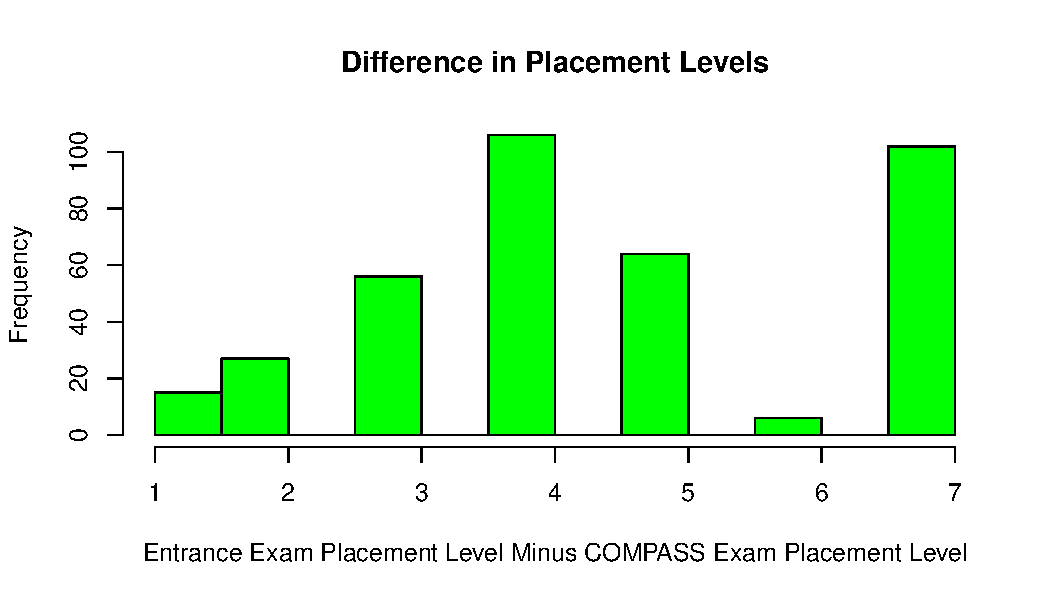
\includegraphics[width=\maxwidth]{figure/histOfLevelsSkipped-1} 

\end{knitrout}


The following table lists the major results of the study.  LEGEND: The first column of each line indicates the course name and the relevant cutoff grade (on a 4.0 scale); EESR is the success rate of students placed by the Entrance Exams, reported as a percent; OSR is the success rate of other students; \#EE is the number of students attempting placement by the corresponding Entrance Exam, and \#O is the number of students placed by other means.  The listed P-value for each class corresponds to an exact binomal test applied to the counts of successful and unsuccessful students placed by Entrance Exams; we use the success rates of students in the corresponding course placed by other means as the parameter for the binomial distribution.

\begin{knitrout}
\definecolor{shadecolor}{rgb}{0.969, 0.969, 0.969}\color{fgcolor}\begin{kframe}
\begin{verbatim}
##                            EESR (%)  OSR (%) #EE   #O P-Value
## Arithmetic (2.5)           56.60377 67.64855  53 1969   0.105
## Prealgebra (2.5)           73.61111 74.04103  72 2242   0.894
## Elementary Algebra (2.5)   73.79310 68.76813 145 5171   0.210
## Intermediate Algebra (2.0) 75.43860 72.61443 228 5156   0.373
## Intermediate Algebra (2.5) 61.84211 64.87587 228 5156   0.332
## Math In Society (1.0)      84.90566 81.84438 106 1041   0.528
## Finite Math (1.0)          84.90566 79.16236 106 1934   0.187
## Finite Math (2.0)          82.07547 69.75181 106 1934   0.006
## Precalculus 1 (1.0)        84.61538 82.17231  78 3517   0.659
## Precalculus 1 (2.0)        80.76923 71.65198  78 3517   0.079
## Precalculus 2 (2.0)        66.66667 73.08869  15 1962   0.566
## Calculus 1 (2.0)           84.81675 73.69104 191 2311   0.000
\end{verbatim}
\end{kframe}
\end{knitrout}


This graph illustrates the success rates listed in the table above.


\begin{knitrout}
\definecolor{shadecolor}{rgb}{0.969, 0.969, 0.969}\color{fgcolor}
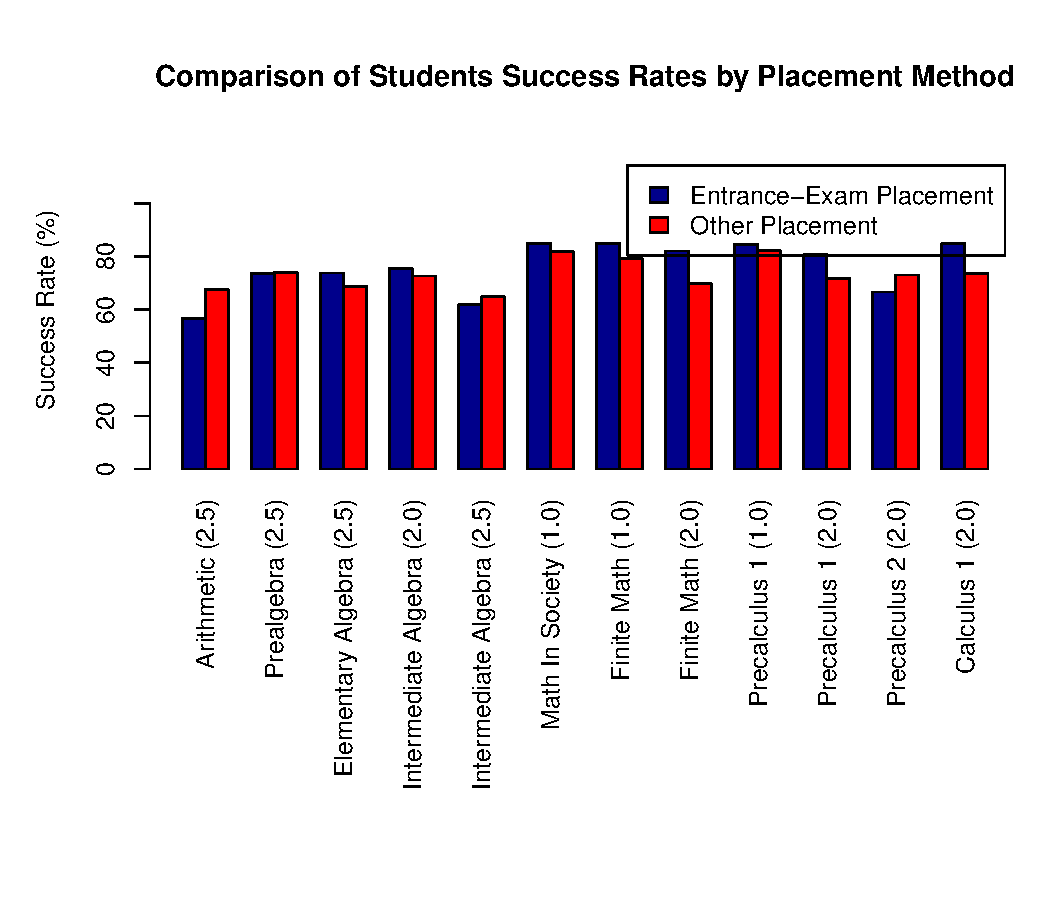
\includegraphics[width=\maxwidth]{figure/success-graphs-1} 

\end{knitrout}

The only statistically significant difference in success rates occurred in the Calculus 1 course, and the success rate there was {\it higher} for students placed by into that course by an Entrance Exams compared to those placed by other means.  (The p-value seen in the Finite Math group should not be considered significant because of the multiple-testing effect.  If we use a standard significance level of $\alpha = 0.05$ for this study of 12 hypotheses, then the Bonferroni correction for multiple testing suggests that the cutoff value for significance in each individual comparison should be $\frac{0.05}{12} \approx 0.004$.)


Taken together, these results suggest that across all levels, the Entrance Exams do no worse in placing the population of students who elect to take them than other placement mechanisms available at the college.


\section{Grade Distributions}

An important question to ask here is whether the population of students who opt to take an Entrance Exam is somehow fundamentally different from the population of students who don't.  That is to say, if the success rates differ, are there counfounding variables that could account for this?  For example, is it possible that students who chose to take an extra test happen to have stonger academic skills to begin with?  We explore several aspects of the available data to try to answer this question.

The following subsections includes graphs that illustrate the distributions of grades for students placed by Entrance Exams and those placed by other means.  In each histogram, the far-left bar represents the combined tally of the non-numerical grades earned: W (withdrawal), I (Incomplete), NC (No Credit) and N (audit); the non-numerical grades P (Pass) are included in the tally with numerical grades of 1.0.

We also examine students' concurrent GPA.  It would seem ideal if we could look only at their GPA in other (non-math) classes, since the overall GPA in a given quarter is of course correlated with the performance in the math class taken at that time; however, it is not possible to extract a grade-point average in their other classes from the information available, because there is no way to determine how many credits we should be dividing by in order to compute the average.  We would need to know the actual grades earned in the other courses.  For example, it makes a difference if a student withdrew form another class rather than earning a 0.0 in it, because that affects the process of the grade-point calculation (credits corresponding to classes from which a student withdraws are not used in computing the average); however that information is not available in this data set.  We will therefore be satisfied with examining the students' overall concurrent GPA while enrolled in a math class, including the math grades.

It is worth noting that, in every course, the mean concurrent GPA was greater among the Entrance-Exam placed students than for other students.  In several of these courses, the difference was statistically significant.  This suggests that there may be a difference in overall academic abilities between students who opt to take an Entrance Exam and those who don't, a possible confounding variable that makes it difficult to predict what would happen with the success rates if the current system of using Entrance Exams as an optional secondary mechanism for placement were to be substantially altered in the future.













\newpage
\subsection{MATH062 - Arithmetic}

\begin{knitrout}
\definecolor{shadecolor}{rgb}{0.969, 0.969, 0.969}\color{fgcolor}
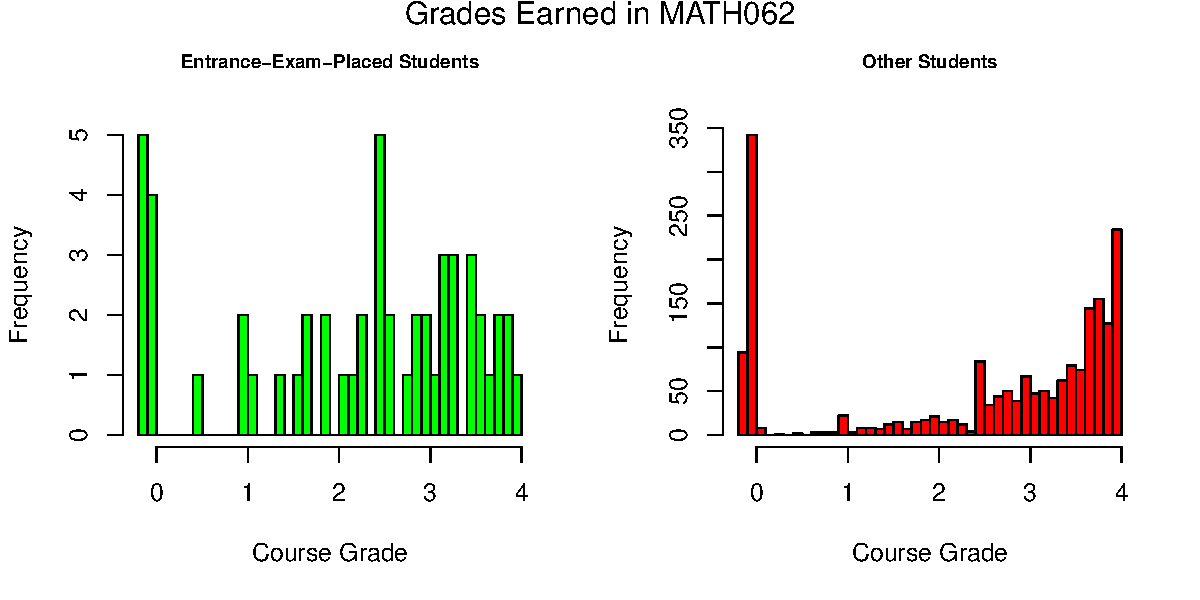
\includegraphics[width=\maxwidth]{figure/graphs062-1} 

\end{knitrout}

Student Success Rates at the 2.5 Grade-Point Level (\%) by Entrance Exam score:

\begin{knitrout}
\definecolor{shadecolor}{rgb}{0.969, 0.969, 0.969}\color{fgcolor}\begin{kframe}
\begin{verbatim}
##               
##                   80    85    90    95    99
##   Unsuccessful  50.0  39.1  40.0 100.0   0.0
##   Successful    50.0  60.9  60.0   0.0 100.0
\end{verbatim}
\end{kframe}
\end{knitrout}


\begin{knitrout}
\definecolor{shadecolor}{rgb}{0.969, 0.969, 0.969}\color{fgcolor}
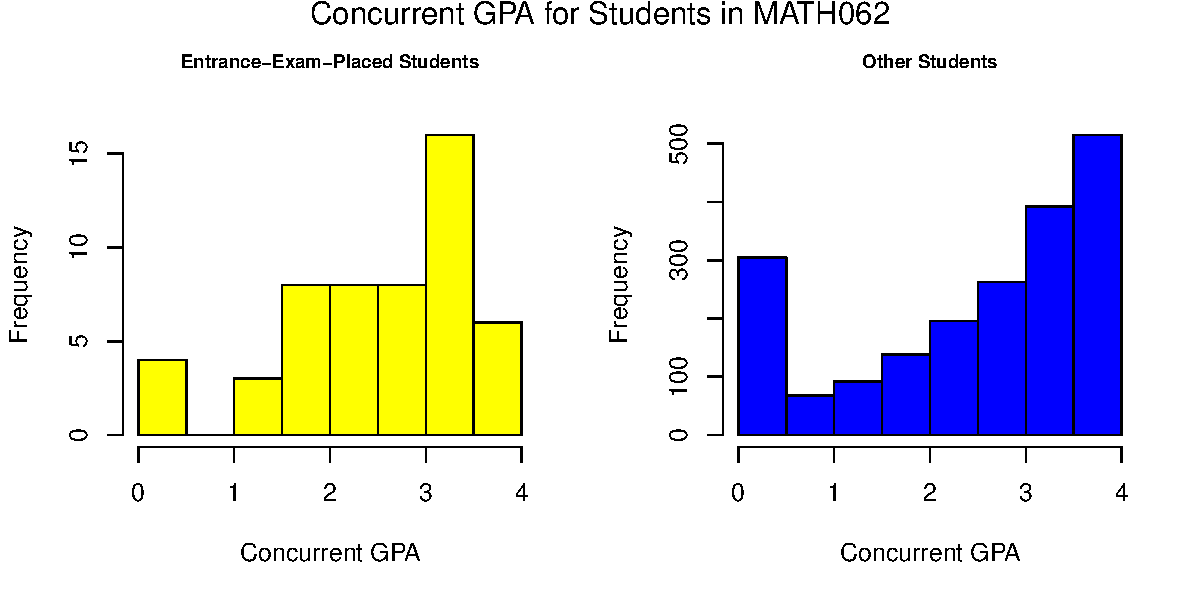
\includegraphics[width=\maxwidth]{figure/GPAgraphs062-1} 

\end{knitrout}

The mean concurrent GPA of students who were placed by Entrance Exam is 2.49, and the mean concurrent GPA of students placed by other means is 2.47.  A T-test of the null hypothesis that the mean concurrent GPA is the same for both groups produces a P-value of 0.846.

\newpage
\subsection{MATH070 - Pre-Algebra}

\begin{knitrout}
\definecolor{shadecolor}{rgb}{0.969, 0.969, 0.969}\color{fgcolor}
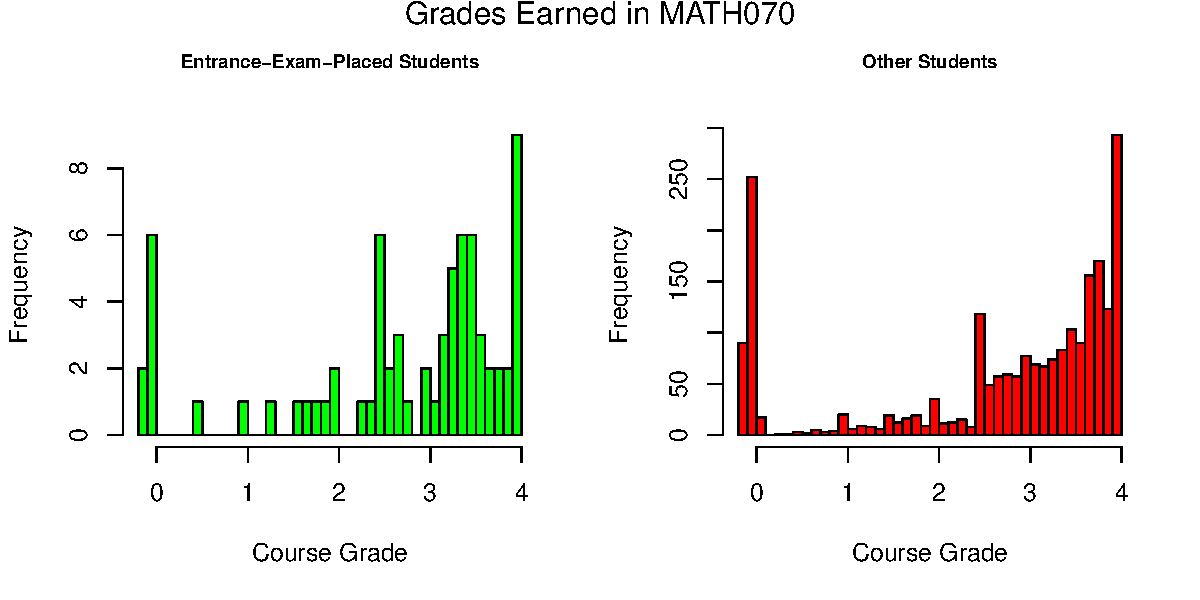
\includegraphics[width=\maxwidth]{figure/graphs070-1} 

\end{knitrout}


Student Success Rates  at the 2.5 Grade-Point Level (\%) by Entrance Exam Score:

\begin{knitrout}
\definecolor{shadecolor}{rgb}{0.969, 0.969, 0.969}\color{fgcolor}\begin{kframe}
\begin{verbatim}
##               
##                  180   185   190   195   199
##   Unsuccessful  37.8 100.0   4.3   0.0  42.9
##   Successful    62.2   0.0  95.7 100.0  57.1
\end{verbatim}
\end{kframe}
\end{knitrout}


\begin{knitrout}
\definecolor{shadecolor}{rgb}{0.969, 0.969, 0.969}\color{fgcolor}
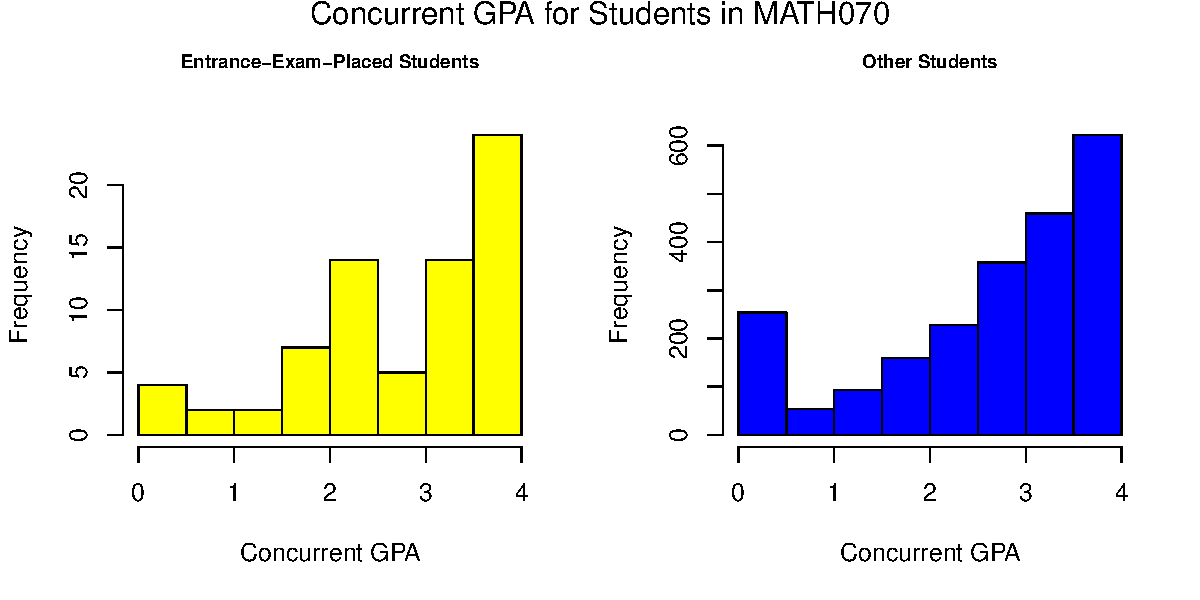
\includegraphics[width=\maxwidth]{figure/GPAgraphs070-1} 

\end{knitrout}

The mean concurrent GPA of students who were placed by Entrance Exam is 2.79, and the mean concurrent GPA of students placed by other means is 2.62.  A T-test of the null hypothesis that the mean concurrent GPA is the same for both groups produces a P-value of 0.201.

\newpage
\subsection{MATH072 - Elementary Algebra}

\begin{knitrout}
\definecolor{shadecolor}{rgb}{0.969, 0.969, 0.969}\color{fgcolor}
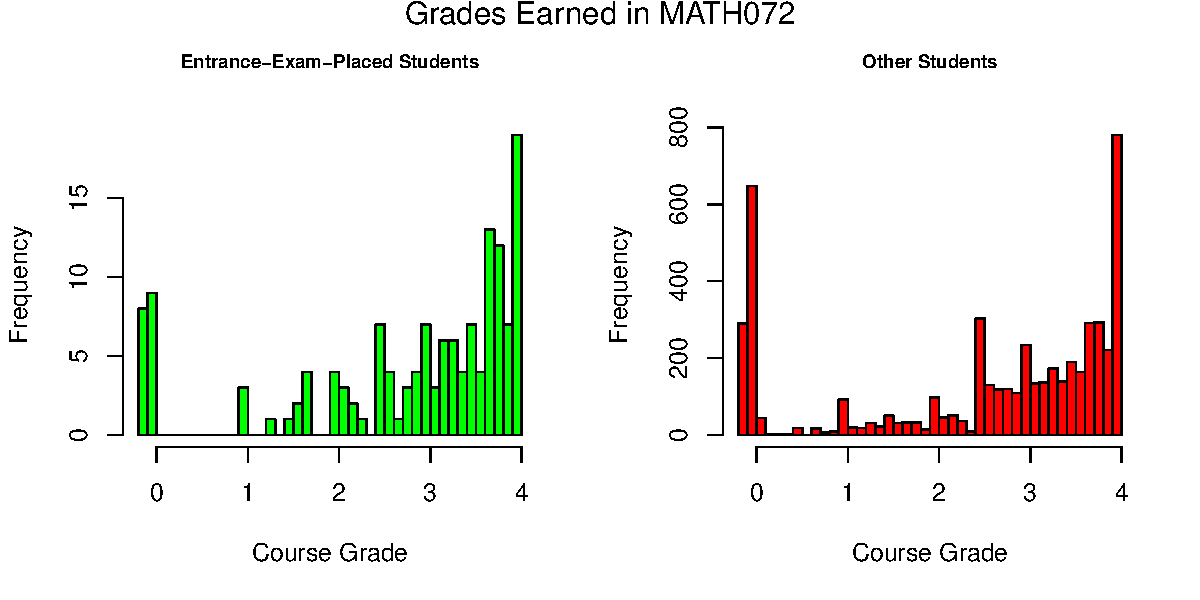
\includegraphics[width=\maxwidth]{figure/graphs072-1} 

\end{knitrout}


Student Success Rates  at the 2.5 Grade-Point Level (\%) by Entrance Exam Score:

\begin{knitrout}
\definecolor{shadecolor}{rgb}{0.969, 0.969, 0.969}\color{fgcolor}\begin{kframe}
\begin{verbatim}
##               
##                 280  285  290  295  299
##   Unsuccessful 20.6 12.5 28.6 37.5 15.4
##   Successful   79.4 87.5 71.4 62.5 84.6
\end{verbatim}
\end{kframe}
\end{knitrout}


\begin{knitrout}
\definecolor{shadecolor}{rgb}{0.969, 0.969, 0.969}\color{fgcolor}
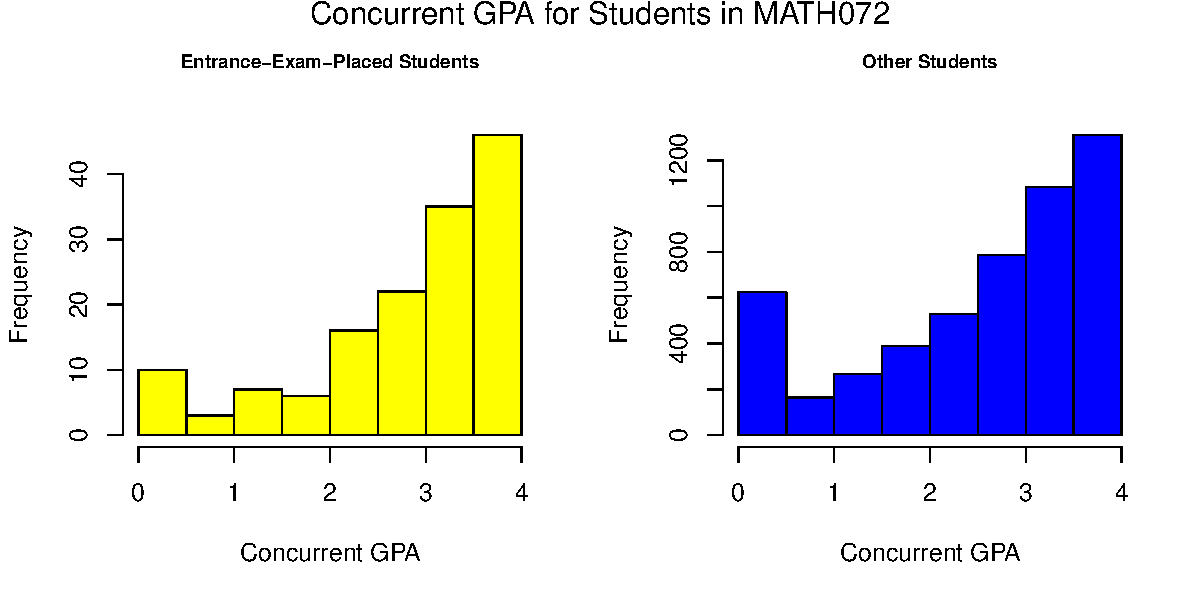
\includegraphics[width=\maxwidth]{figure/GPAgraphs072-1} 

\end{knitrout}

The mean concurrent GPA of students who were placed by Entrance Exam is 2.85, and the mean concurrent GPA of students placed by other means is 2.55.  A T-test of the null hypothesis that the mean concurrent GPA is the same for both groups produces a P-value of 0.001.

\newpage
\subsection{MATH097 - Intermediate Algebra}

\begin{knitrout}
\definecolor{shadecolor}{rgb}{0.969, 0.969, 0.969}\color{fgcolor}
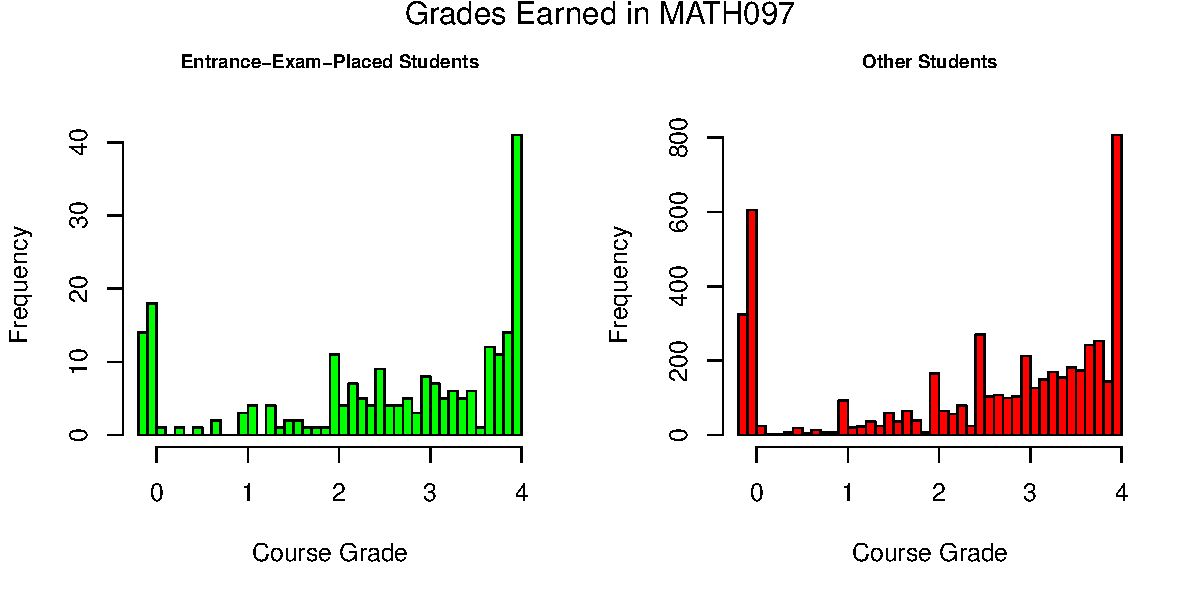
\includegraphics[width=\maxwidth]{figure/graphs097-1} 

\end{knitrout}



Student Success Rates  at the 2.5 Grade-Point Level (\%) by Entrance Exam Score:

\begin{knitrout}
\definecolor{shadecolor}{rgb}{0.969, 0.969, 0.969}\color{fgcolor}\begin{kframe}
\begin{verbatim}
##               
##                  380   382   383   385   388   390   395   398   399
##   Unsuccessful  43.5  33.3   0.0  46.7 100.0  26.8  32.5  50.0   0.0
##   Successful    56.5  66.7 100.0  53.3   0.0  73.2  67.5  50.0 100.0
\end{verbatim}
\end{kframe}
\end{knitrout}

Student Success Rates  at the 2.0 Grade-Point Level (\%) by Entrance Exam Score:

\begin{knitrout}
\definecolor{shadecolor}{rgb}{0.969, 0.969, 0.969}\color{fgcolor}\begin{kframe}
\begin{verbatim}
##               
##                  380   382   383   385   388   390   395   398   399
##   Unsuccessful  25.8  33.3   0.0  33.3 100.0  14.3  20.0  50.0   0.0
##   Successful    74.2  66.7 100.0  66.7   0.0  85.7  80.0  50.0 100.0
\end{verbatim}
\end{kframe}
\end{knitrout}


\begin{knitrout}
\definecolor{shadecolor}{rgb}{0.969, 0.969, 0.969}\color{fgcolor}
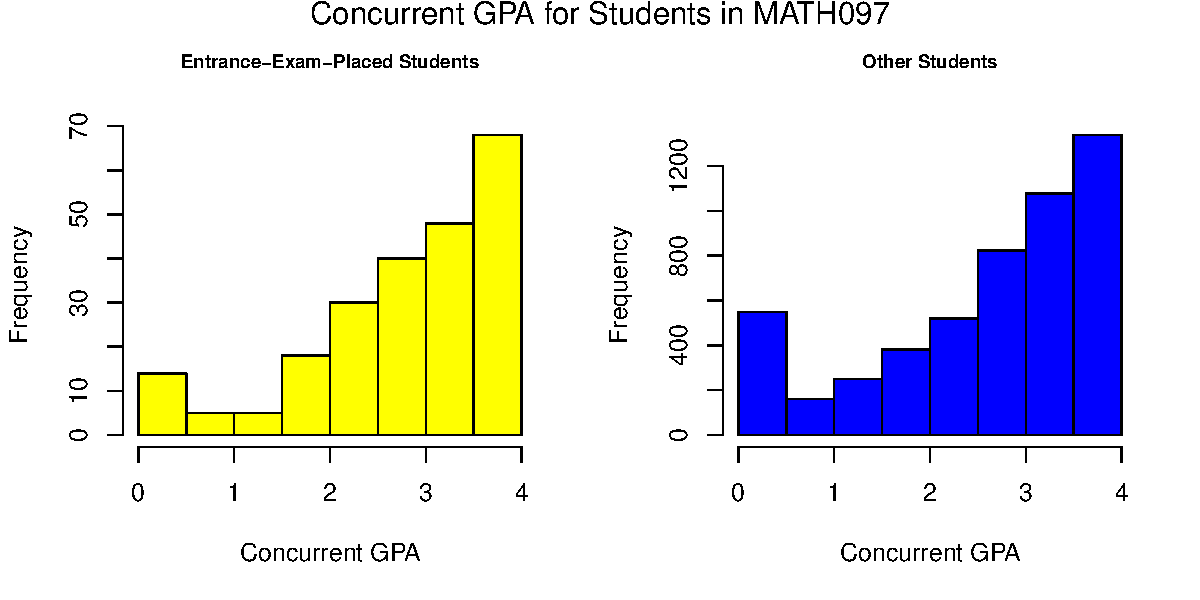
\includegraphics[width=\maxwidth]{figure/GPAgraphs097-1} 

\end{knitrout}

The mean concurrent GPA of students who were placed by Entrance Exam is 2.82, and the mean concurrent GPA of students placed by other means is 2.6.  A T-test of the null hypothesis that the mean concurrent GPA is the same for both groups produces a P-value of 0.003.


\newpage
\subsection{MATH\&107 - Math in Society}

\begin{knitrout}
\definecolor{shadecolor}{rgb}{0.969, 0.969, 0.969}\color{fgcolor}
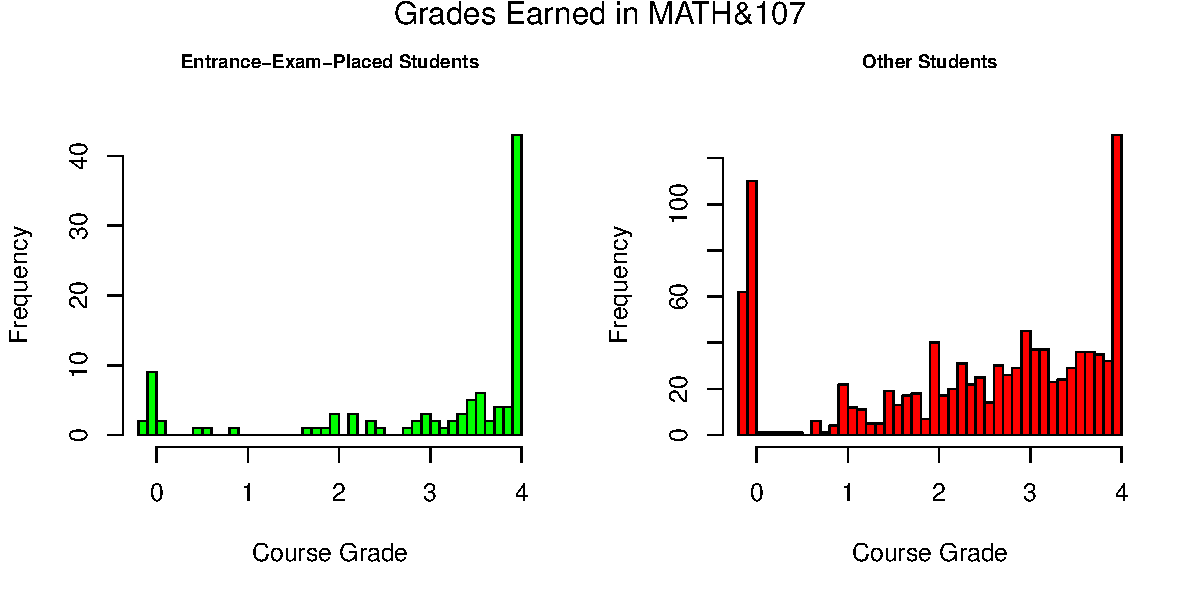
\includegraphics[width=\maxwidth]{figure/graphs107-1} 

\end{knitrout}


Student Success Rates  at the 1.0 Grade-Point Level (\%) by Entrance Exam Score:

\begin{knitrout}
\definecolor{shadecolor}{rgb}{0.969, 0.969, 0.969}\color{fgcolor}\begin{kframe}
\begin{verbatim}
##               
##                  475   476   478   480   481   482   483   485   486   488
##   Unsuccessful  16.7   0.0  14.3  13.3   0.0   0.0  18.2   8.3   0.0  40.0
##   Successful    83.3 100.0  85.7  86.7 100.0 100.0  81.8  91.7 100.0  60.0
##               
##                  490   495
##   Unsuccessful  16.7  25.0
##   Successful    83.3  75.0
\end{verbatim}
\end{kframe}
\end{knitrout}


\begin{knitrout}
\definecolor{shadecolor}{rgb}{0.969, 0.969, 0.969}\color{fgcolor}
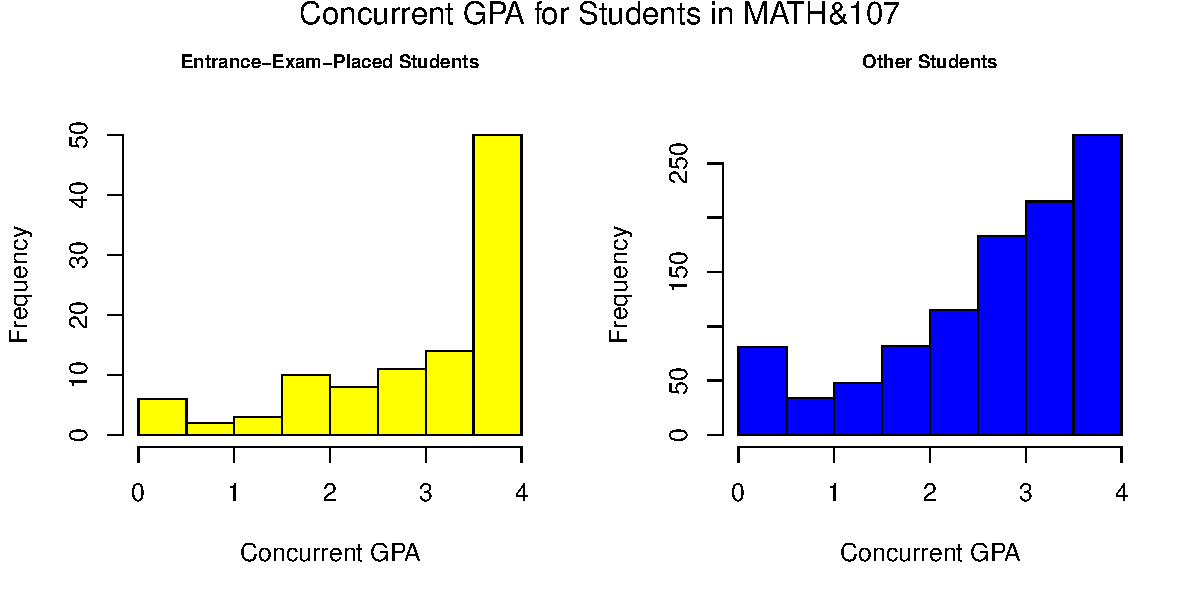
\includegraphics[width=\maxwidth]{figure/GPAgraphs107-1} 

\end{knitrout}

The mean concurrent GPA of students who were placed by Entrance Exam is 2.99, and the mean concurrent GPA of students placed by other means is 2.68.  A T-test of the null hypothesis that the mean concurrent GPA is the same for both groups produces a P-value of 0.007.



\newpage
\subsection{MATH147 - Finite Math for Business and Social Science}

\begin{knitrout}
\definecolor{shadecolor}{rgb}{0.969, 0.969, 0.969}\color{fgcolor}
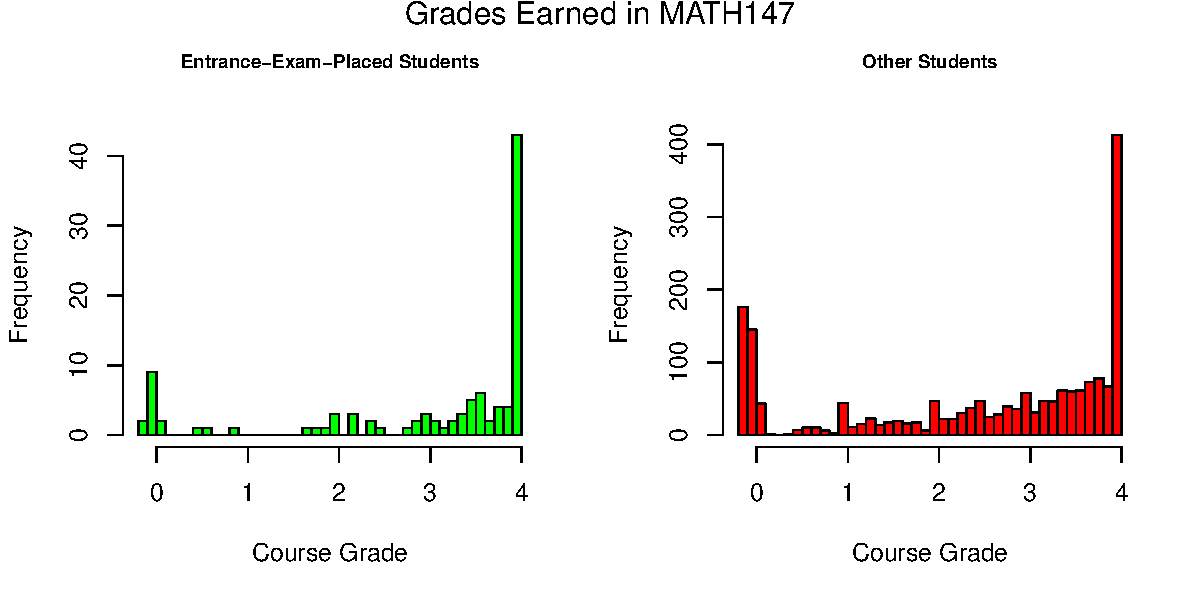
\includegraphics[width=\maxwidth]{figure/graphs147-1} 

\end{knitrout}


Student Success Rates  at the 1.0 Grade-Point Level (\%) by Entrance Exam Score:

\begin{knitrout}
\definecolor{shadecolor}{rgb}{0.969, 0.969, 0.969}\color{fgcolor}\begin{kframe}
\begin{verbatim}
##               
##                  475   476   478   480   481   482   483   485   486   488
##   Unsuccessful  16.7   0.0  14.3  13.3   0.0   0.0  18.2   8.3   0.0  40.0
##   Successful    83.3 100.0  85.7  86.7 100.0 100.0  81.8  91.7 100.0  60.0
##               
##                  490   495
##   Unsuccessful  16.7  25.0
##   Successful    83.3  75.0
\end{verbatim}
\end{kframe}
\end{knitrout}


Student Success Rates  at the 2.0 Grade-Point Level (\%) by Entrance Exam Score:

\begin{knitrout}
\definecolor{shadecolor}{rgb}{0.969, 0.969, 0.969}\color{fgcolor}\begin{kframe}
\begin{verbatim}
##               
##                  475   476   478   480   481   482   483   485   486   488
##   Unsuccessful  16.7   0.0  14.3  20.0  50.0   0.0  18.2   8.3   0.0  40.0
##   Successful    83.3 100.0  85.7  80.0  50.0 100.0  81.8  91.7 100.0  60.0
##               
##                  490   495
##   Unsuccessful  16.7  25.0
##   Successful    83.3  75.0
\end{verbatim}
\end{kframe}
\end{knitrout}


\begin{knitrout}
\definecolor{shadecolor}{rgb}{0.969, 0.969, 0.969}\color{fgcolor}
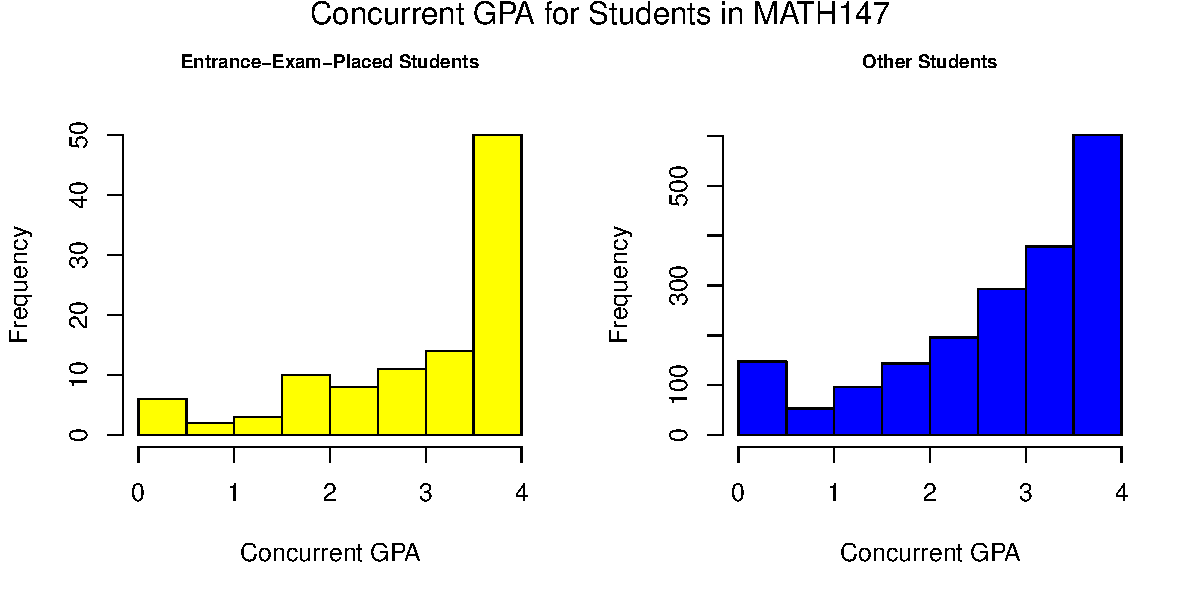
\includegraphics[width=\maxwidth]{figure/GPAgraphs147-1} 

\end{knitrout}

The mean concurrent GPA of students who were placed by Entrance Exam is 2.99, and the mean concurrent GPA of students placed by other means is 2.74.  A T-test of the null hypothesis that the mean concurrent GPA is the same for both groups produces a P-value of 0.028.


\newpage
\subsection{MATH\&141 - Precalculus 1}

\begin{knitrout}
\definecolor{shadecolor}{rgb}{0.969, 0.969, 0.969}\color{fgcolor}
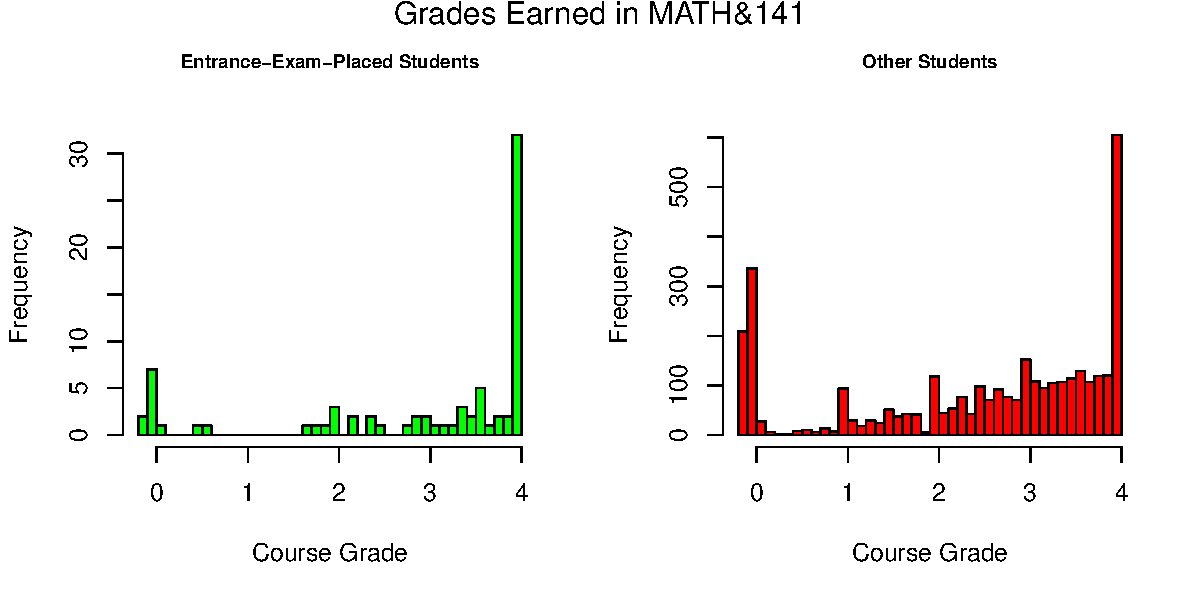
\includegraphics[width=\maxwidth]{figure/graphs141-1} 

\end{knitrout}

Student Success Rates  at the 1.0 Grade-Point Level (\%) by Entrance Exam Score:

\begin{knitrout}
\definecolor{shadecolor}{rgb}{0.969, 0.969, 0.969}\color{fgcolor}\begin{kframe}
\begin{verbatim}
##               
##                  480   481   482   483   485   486   488   490   495
##   Unsuccessful  13.3   0.0   0.0  18.2   8.3   0.0  40.0  16.7  25.0
##   Successful    86.7 100.0 100.0  81.8  91.7 100.0  60.0  83.3  75.0
\end{verbatim}
\end{kframe}
\end{knitrout}


Student Success Rates  at the 2.0 Grade-Point Level (\%) by Entrance Exam Score:

\begin{knitrout}
\definecolor{shadecolor}{rgb}{0.969, 0.969, 0.969}\color{fgcolor}\begin{kframe}
\begin{verbatim}
##               
##                  480   481   482   483   485   486   488   490   495
##   Unsuccessful  20.0  50.0   0.0  18.2   8.3   0.0  40.0  16.7  25.0
##   Successful    80.0  50.0 100.0  81.8  91.7 100.0  60.0  83.3  75.0
\end{verbatim}
\end{kframe}
\end{knitrout}


\begin{knitrout}
\definecolor{shadecolor}{rgb}{0.969, 0.969, 0.969}\color{fgcolor}
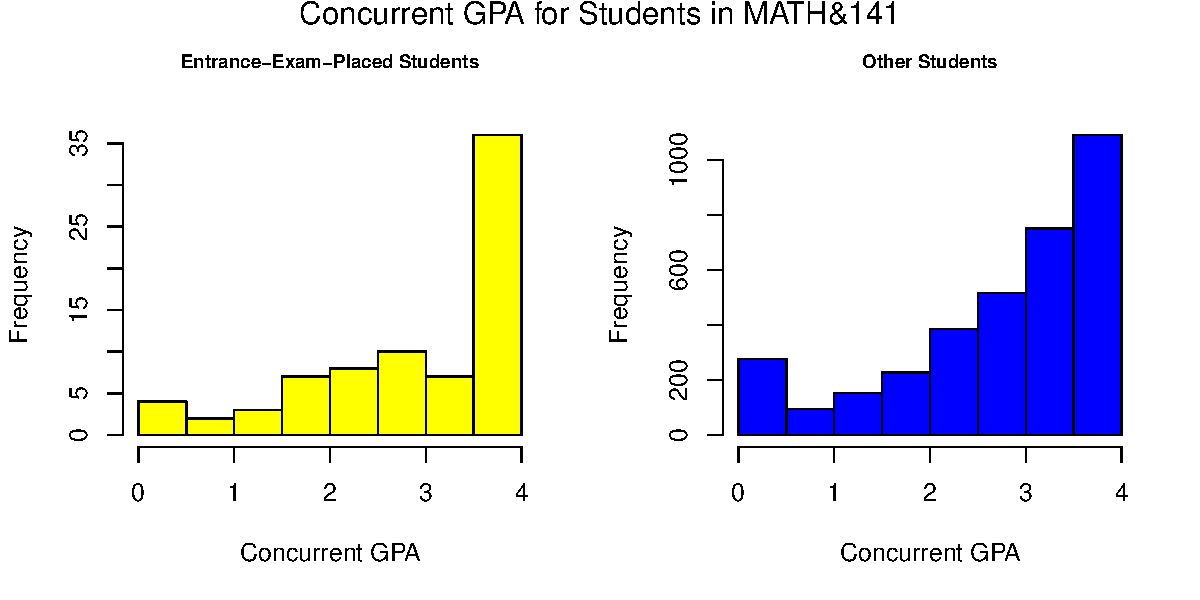
\includegraphics[width=\maxwidth]{figure/GPAgraphs141-1} 

\end{knitrout}

The mean concurrent GPA of students who were placed by Entrance Exam is 2.93, and the mean concurrent GPA of students placed by other means is 2.75.  A T-test of the null hypothesis that the mean concurrent GPA is the same for both groups produces a P-value of 0.17.



\newpage
\subsection{MATH\&142 - Precalculus 2}


\begin{knitrout}
\definecolor{shadecolor}{rgb}{0.969, 0.969, 0.969}\color{fgcolor}
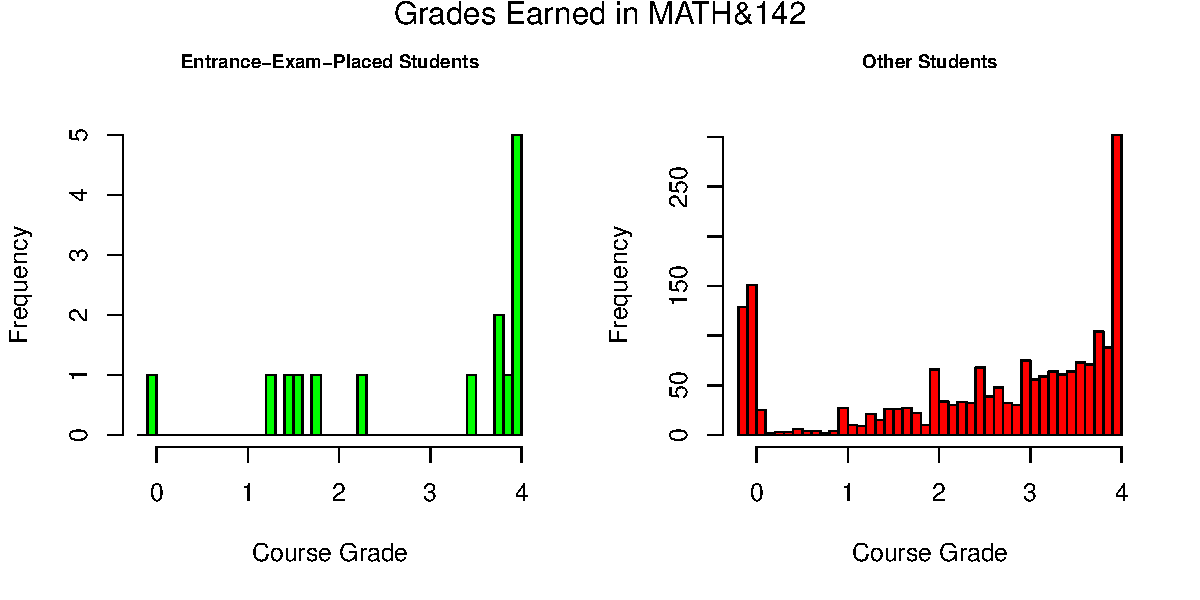
\includegraphics[width=\maxwidth]{figure/graphs142-1} 

\end{knitrout}



Student Success Rates  at the 2.0 Grade-Point Level (\%) by Entrance Exam Score:

\begin{knitrout}
\definecolor{shadecolor}{rgb}{0.969, 0.969, 0.969}\color{fgcolor}\begin{kframe}
\begin{verbatim}
##               
##                  575   577   578   580
##   Unsuccessful   0.0   0.0  50.0  57.1
##   Successful   100.0 100.0  50.0  42.9
\end{verbatim}
\end{kframe}
\end{knitrout}


\begin{knitrout}
\definecolor{shadecolor}{rgb}{0.969, 0.969, 0.969}\color{fgcolor}
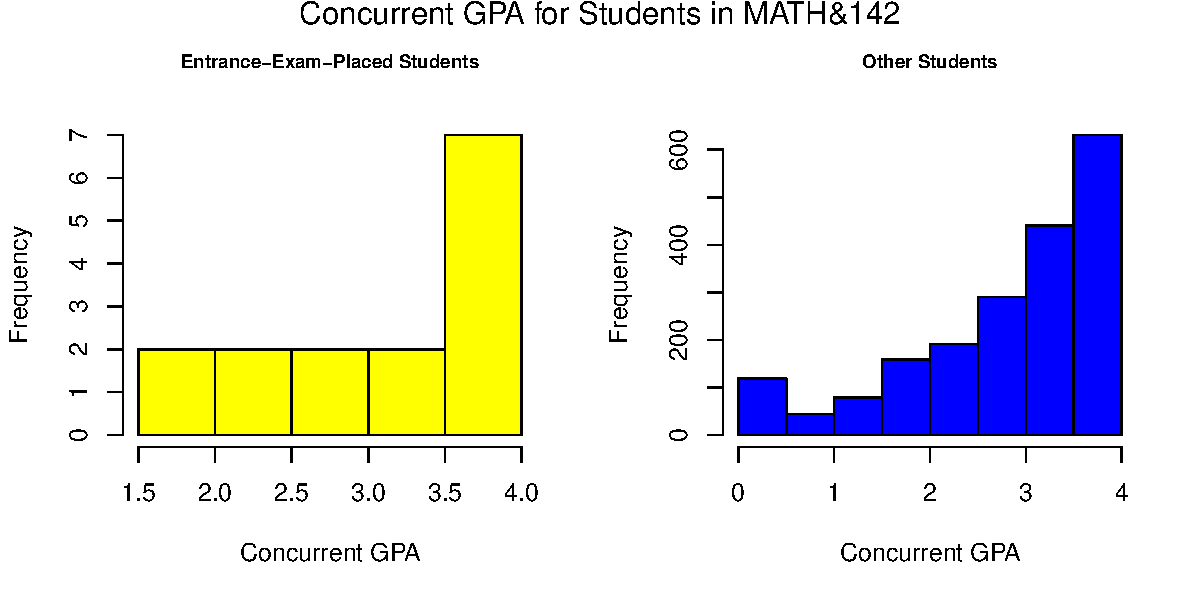
\includegraphics[width=\maxwidth]{figure/GPAgraphs142-1} 

\end{knitrout}

The mean concurrent GPA of students who were placed by Entrance Exam is 3.13, and the mean concurrent GPA of students placed by other means is 2.82.  A T-test of the null hypothesis that the mean concurrent GPA is the same for both groups produces a P-value of 0.17.





\newpage
\subsection{MATH\&151 - Calculus 1}


\begin{knitrout}
\definecolor{shadecolor}{rgb}{0.969, 0.969, 0.969}\color{fgcolor}
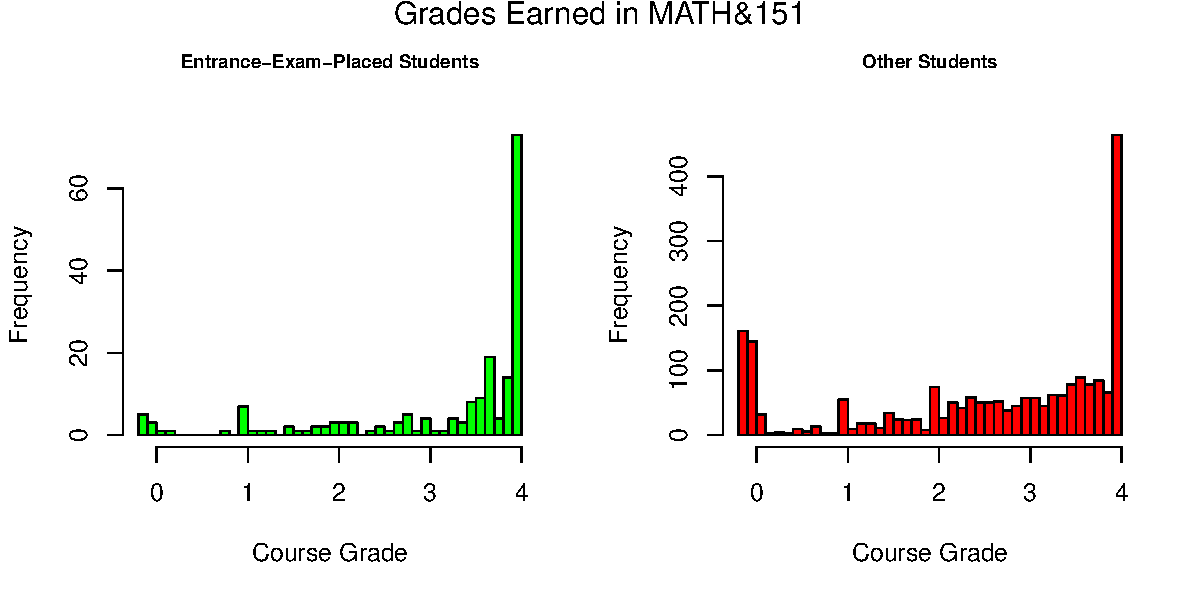
\includegraphics[width=\maxwidth]{figure/graphs151-1} 

\end{knitrout}


Student Success Rates  at the 2.0 Grade-Point Level (\%) by Entrance Exam Score:

\begin{knitrout}
\definecolor{shadecolor}{rgb}{0.969, 0.969, 0.969}\color{fgcolor}\begin{kframe}
\begin{verbatim}
##               
##                  675   676   677   678   679   680   682   683   685   686
##   Unsuccessful  21.3   0.0  12.5   0.0   0.0  16.7   0.0   0.0  13.6   0.0
##   Successful    78.7 100.0  87.5 100.0 100.0  83.3 100.0 100.0  86.4 100.0
##               
##                  687   688   689   690   692   694   695   697
##   Unsuccessful   0.0   0.0  33.3  21.4   0.0  25.0  12.5   0.0
##   Successful   100.0 100.0  66.7  78.6 100.0  75.0  87.5 100.0
\end{verbatim}
\end{kframe}
\end{knitrout}


\begin{knitrout}
\definecolor{shadecolor}{rgb}{0.969, 0.969, 0.969}\color{fgcolor}
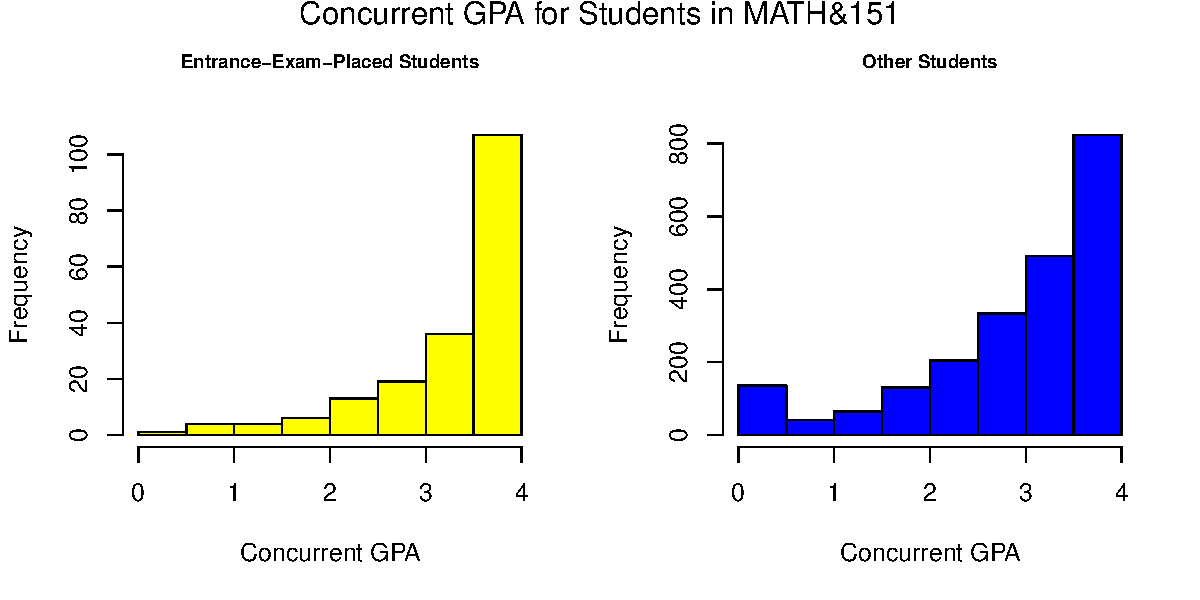
\includegraphics[width=\maxwidth]{figure/GPAgraphs151-1} 

\end{knitrout}

The mean concurrent GPA of students who were placed by Entrance Exam is 3.31, and the mean concurrent GPA of students placed by other means is 2.92.  A T-test of the null hypothesis that the mean concurrent GPA is the same for both groups produces a P-value of 0.




\section{Cutoff Scores}


Because the success rates for students placed by the Entrance Exams was often higher than that for students placed by other means, a reasonable question to ask is whether those students who narrowly missed the cutoffs might have been successful as well; if so, then it might be possible to lower the cutoff scores, thus shortening the sequence of math classes necessary for students to complete their educational programs.

This is a complicated question to answer because we don't know exactly how students would have performed in that circumstance.  

%In the graphs below, we explore the grades of students who took a given Entrance Exam and earned scores that were slightly below the cutoff (a difference in score of up to 5 points -- the equivalent of missing one additional question).  We look at their performances in both classes -- the course they attempted to bypass as well as the one into which they attempted to place by the Entrance Exam.

%There is a potential for a lot of noise in this analysis: A student who doesn't meet the necessary grade to move on to the next course in a sequence might attempt to gain entry to that course by taking an Entrance Exam, and because we do not have date information available in our data set that would allow us to distinguish these cases, they could cause some misleading results.  Furthermore, there should be some students who enrolled in classes toward the end of the period of this study, and if they eventually took their desired course after the end of this period, it will not show up in these results.  Consequently, this part of the analysis is purely exploratory.


A promising line of reasoning is to use linear regression to try to predict the grades earned by students as a function of their Entrance Exam scores.  The plan then would be to estimate from the regression whether students achieving a score slightly lower than the current cutoff score would 
be projected to earn a grade that is passing.  

This approach would be absolutely accceptable if we knew that the grade earned is well-correlated with the Entrance Exam score, but as is visible in the scatter plots included here, that is not typically the case.  Indeed, Entrance Exams are not designed to be predictive of the grade a student will earn. Rather, they are meant to indicate whether a student has sufficient comfort with the background material to have a reasonable chance of success in a course.  In fact, in some of the regressions performed here, the correlation between Entrance Exam score and grade earned surprisingly ends up being negative.  (Perhaps unsurprisingly, those negative correlations show up when the sample sizes are very small.)

On the other hand, even though the linear regression is not a perfect predictor of the grade a student will earn, our data shows that, in all of the courses studied, it is a reasonable conservative estimate.  We included histograms of the residuals for the regression models to illustrate this.  If the linear regression were a good predictor of the grade, we would expect to see these residuals be distributed normally, and they are not.  However, in most of the courses, the majority of students performed better than the regression would have predicted from their Entrance Exam score alone.

Based on these results, it seems likely that the Green River College mathematics division could lower the cutoff scores slightly (by 5 points, an amount that permits one additional incorrect exam answer) for passing each of the Entrance Exams without substantial adverse effects on the success rates for students.





\newpage
\subsection{MATH062 - Arithmetic}

















\begin{knitrout}
\definecolor{shadecolor}{rgb}{0.969, 0.969, 0.969}\color{fgcolor}
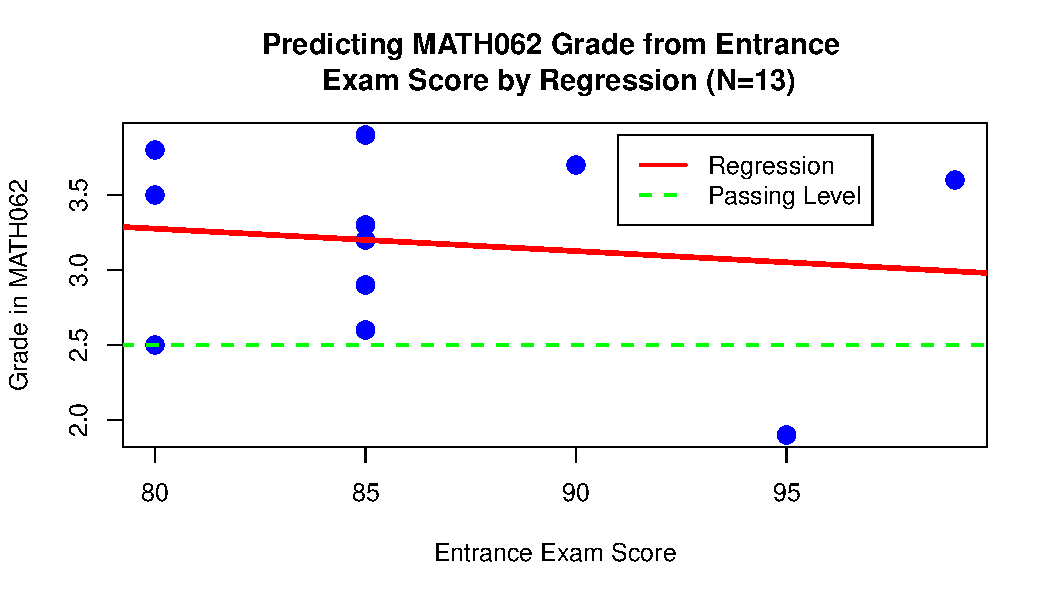
\includegraphics[width=\maxwidth]{figure/062regressiongraph-1} 

\end{knitrout}




\begin{knitrout}
\definecolor{shadecolor}{rgb}{0.969, 0.969, 0.969}\color{fgcolor}
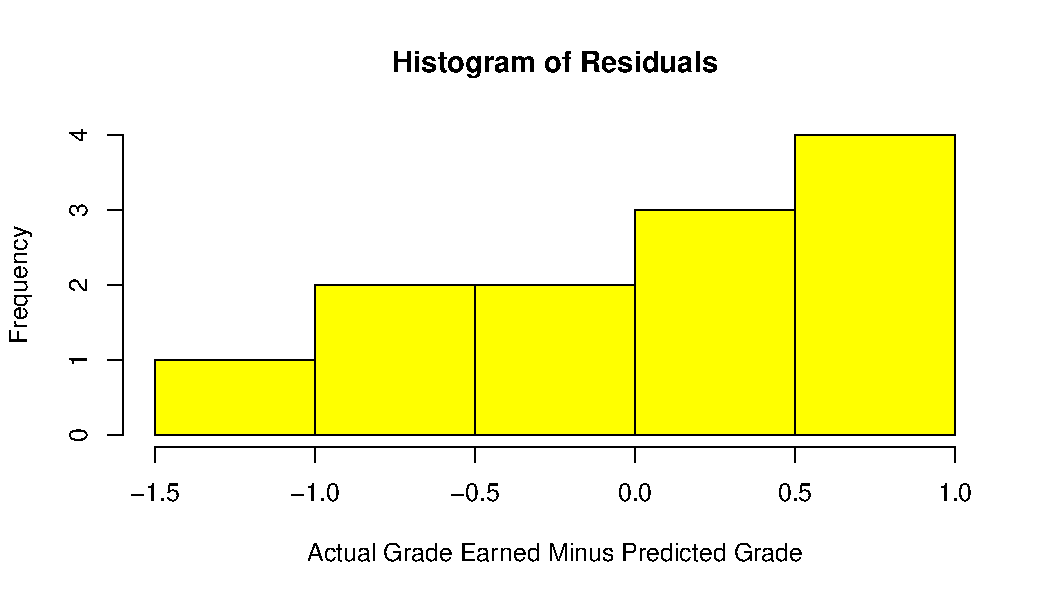
\includegraphics[width=\maxwidth]{figure/062residualsplot-1} 

\end{knitrout}

%There were nearMissesFor062 students who were within 5 points of passing the Entrance Exam for gaining admittance to MATH062.  Students who are not eligible for MATH062 (Arithmetic) may enroll in an Adult Basic Education course (ABE053); passing that course gives students eligibility for MATH062.  Grade data for the ABE course was not included in this study. 

The regression line predicts a grade of 3.3 for a student earning an Entrance Exam score that is 5 points lower than the current cutoff.  The negative slope of this line is likely due to the small sample size and the presence of a single outlier on the bottom right.


\newpage
\subsection{MATH070 - Prealgebra}

%<<070cutoff, echo=FALSE, fig.height=4>>=
%visualDisplayCutoffData(df1, "MATH070", 2.5, "MATH062", 2.5, 180)
%@

\begin{knitrout}
\definecolor{shadecolor}{rgb}{0.969, 0.969, 0.969}\color{fgcolor}
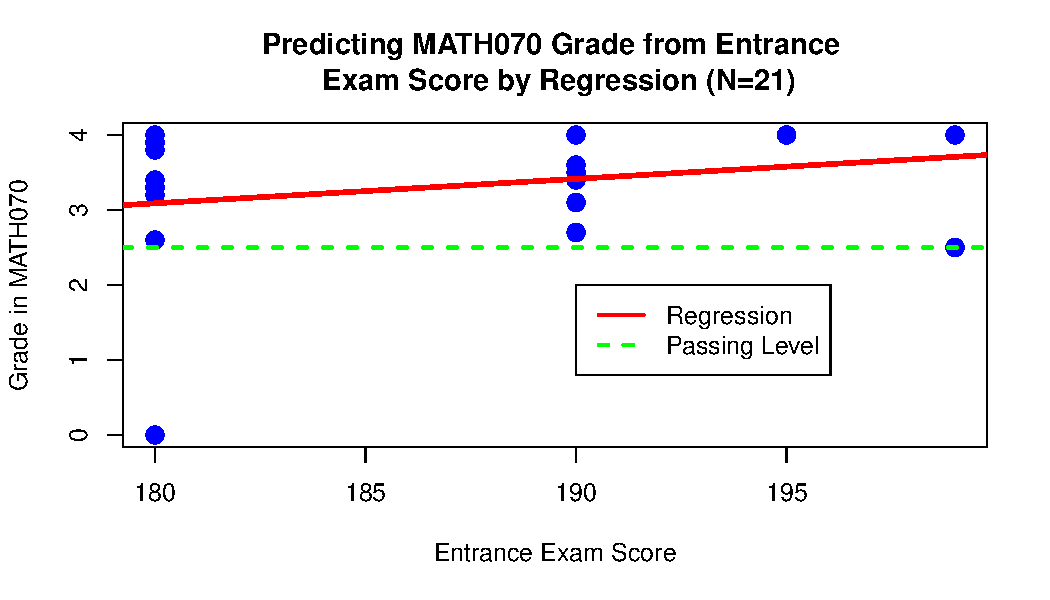
\includegraphics[width=\maxwidth]{figure/070regressiongraph-1} 

\end{knitrout}

\begin{knitrout}
\definecolor{shadecolor}{rgb}{0.969, 0.969, 0.969}\color{fgcolor}
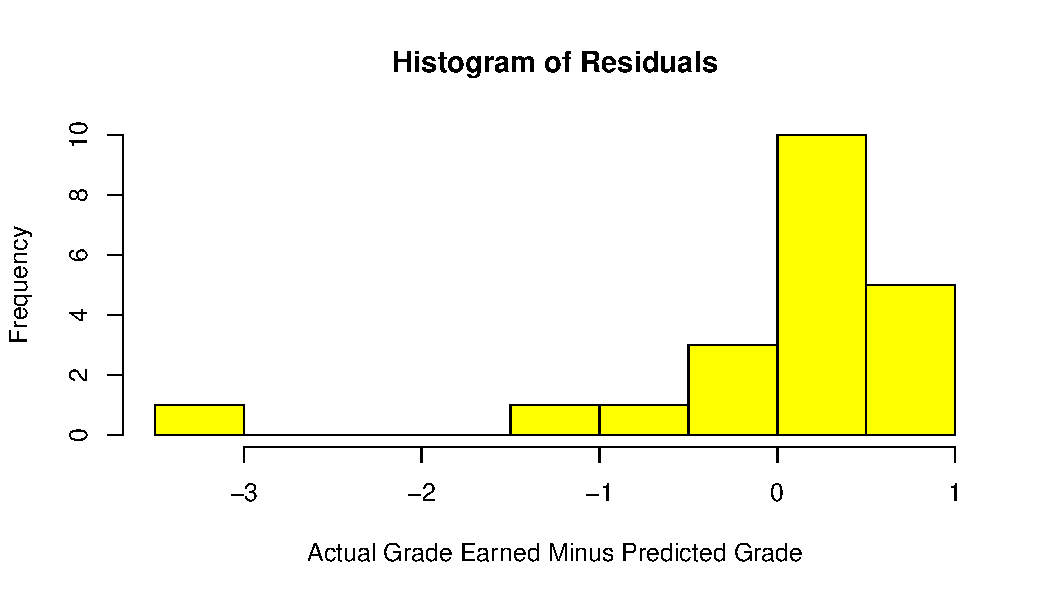
\includegraphics[width=\maxwidth]{figure/070residualsplot-1} 

\end{knitrout}

The regression line predicts a grade of 2.9 for a student earning an Entrance Exam score that is 5 points lower than the current cutoff.



\newpage
\subsection{MATH072 - Elementary Algebra}

%<<072cutoff, echo=FALSE, fig.height=4>>=
%visualDisplayCutoffData(df1, "MATH072", 2.5, "MATH070", 2.5, 280)
%@

\begin{knitrout}
\definecolor{shadecolor}{rgb}{0.969, 0.969, 0.969}\color{fgcolor}
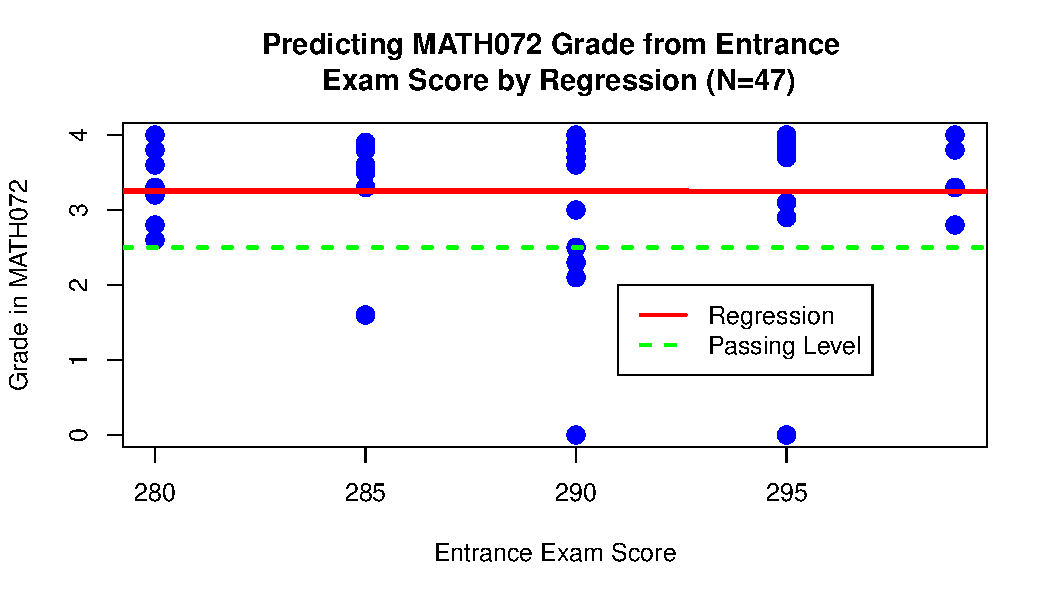
\includegraphics[width=\maxwidth]{figure/072regressiongraph-1} 

\end{knitrout}

\begin{knitrout}
\definecolor{shadecolor}{rgb}{0.969, 0.969, 0.969}\color{fgcolor}
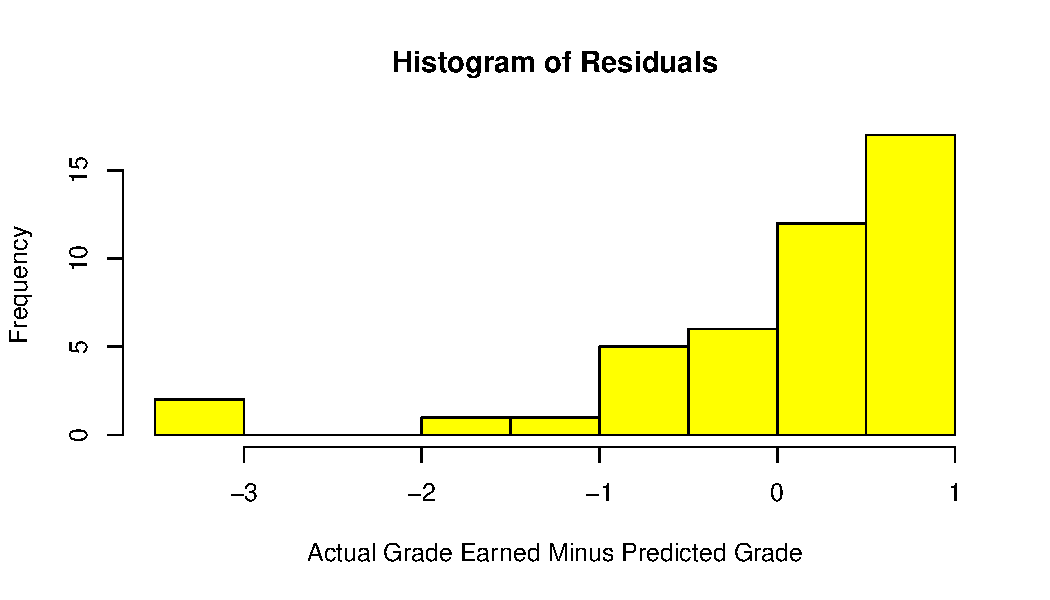
\includegraphics[width=\maxwidth]{figure/072residualsplot-1} 

\end{knitrout}

The regression line predicts a grade of 3.3 for a student earning an Entrance Exam score that is 5 points lower than the current cutoff.



\newpage
\subsection{MATH097 - Intermediate Algebra}

%<<097cutoff, echo=FALSE, fig.height=4>>=
%visualDisplayCutoffData(df1, "MATH097", 2.5, "MATH072", 2.5, 380, textScale = 0.75)
%
%visualDisplayCutoffData(df1, "MATH097", 2.0, "MATH072", 2.5, 380, textScale = 0.75)
%@

\begin{knitrout}
\definecolor{shadecolor}{rgb}{0.969, 0.969, 0.969}\color{fgcolor}
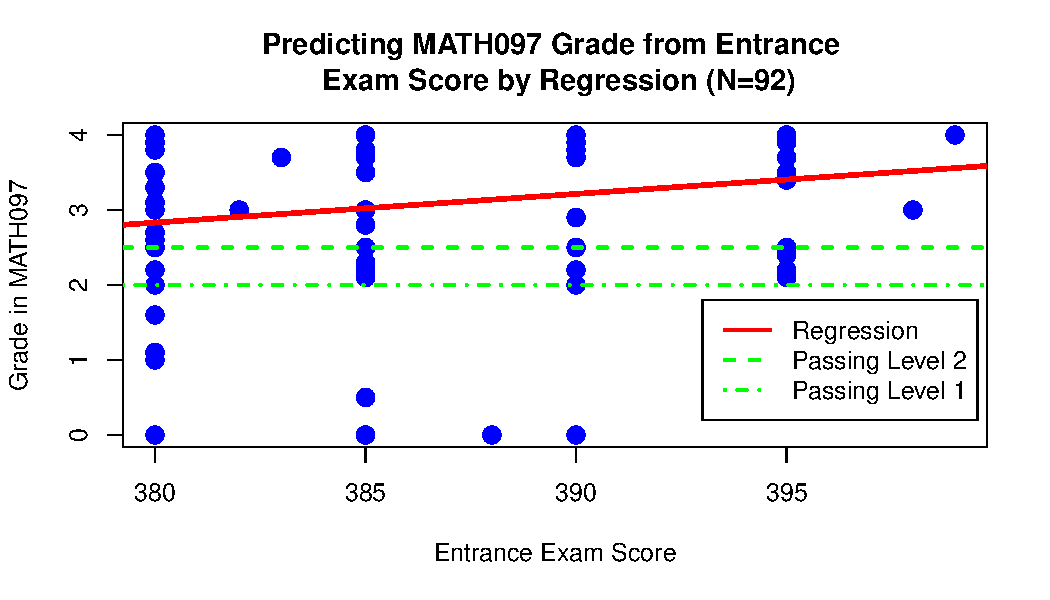
\includegraphics[width=\maxwidth]{figure/097regressiongraph-1} 

\end{knitrout}

\begin{knitrout}
\definecolor{shadecolor}{rgb}{0.969, 0.969, 0.969}\color{fgcolor}
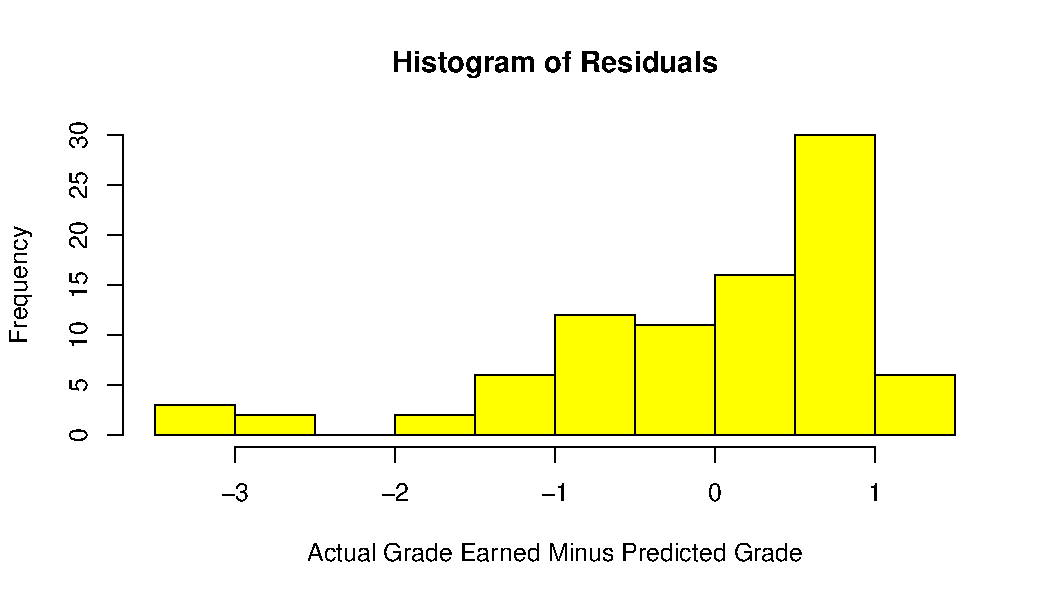
\includegraphics[width=\maxwidth]{figure/097residualsplot-1} 

\end{knitrout}

The regression line predicts a grade of 2.6 for a student earning an Entrance Exam score that is 5 points lower than the current cutoff.


\newpage
\subsection{MATH\&107 - Math in Society}


%<<107cutoff, echo=FALSE, fig.height=4>>=
%visualDisplayCutoffData(df1, "MATH&107", 1.0, "MATH097", 2.0, 475)
%@

\begin{knitrout}
\definecolor{shadecolor}{rgb}{0.969, 0.969, 0.969}\color{fgcolor}
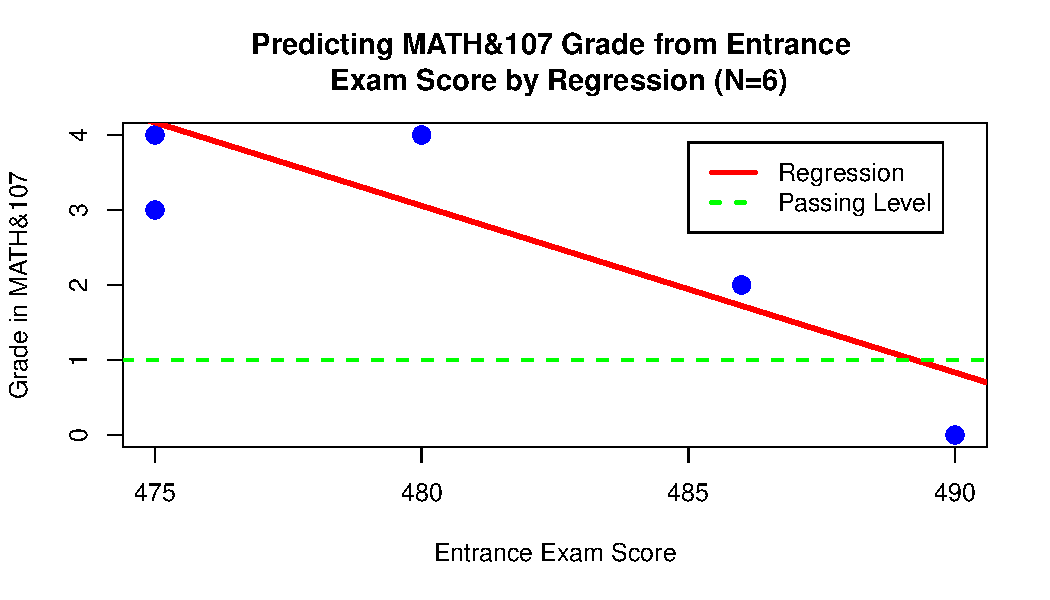
\includegraphics[width=\maxwidth]{figure/107regressiongraph-1} 

\end{knitrout}

\begin{knitrout}
\definecolor{shadecolor}{rgb}{0.969, 0.969, 0.969}\color{fgcolor}
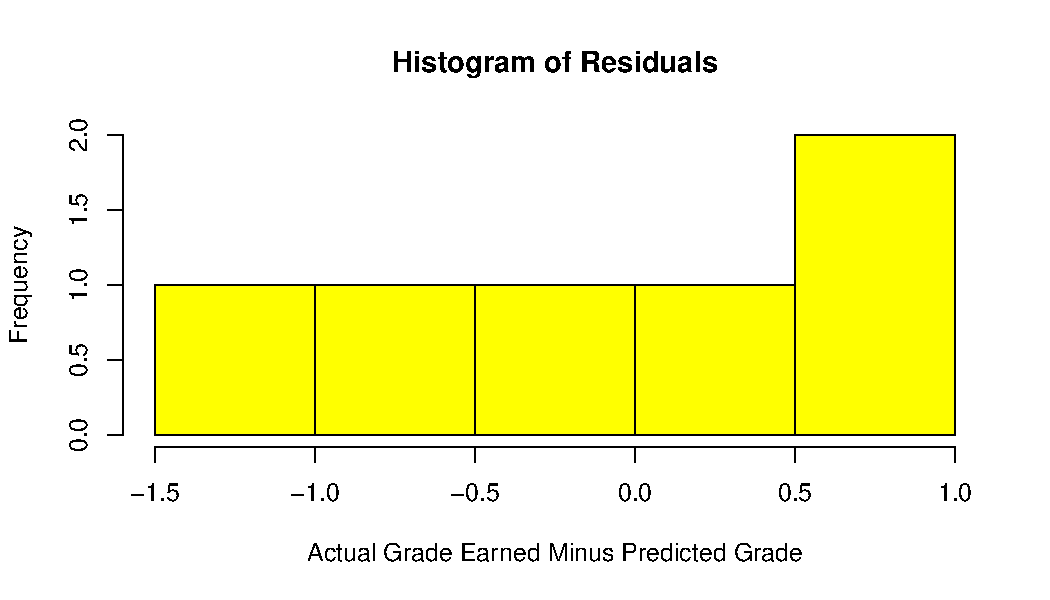
\includegraphics[width=\maxwidth]{figure/107residualsplot-1} 

\end{knitrout}

The regression line predicts a grade of 5.3 for a student earning an Entrance Exam score that is 5 points lower than the current cutoff.  Of course, the maximum possible grade is  4.0.  The negative slope of this line is likely due to the small sample size and the presence of a single outlier on the bottom right.

\newpage
\subsection{MATH\&147 - Finite Math for Business and Social Science}


%<<147cutoff, echo=FALSE, fig.height=4>>=
%visualDisplayCutoffData(df1, "MATH147", 2.0, "MATH097", 2.0, 475, textScale = 0.75)
%
%visualDisplayCutoffData(df1, "MATH147", 1.0, "MATH097", 2.0, 475, textScale = 0.75)
%@

\begin{knitrout}
\definecolor{shadecolor}{rgb}{0.969, 0.969, 0.969}\color{fgcolor}
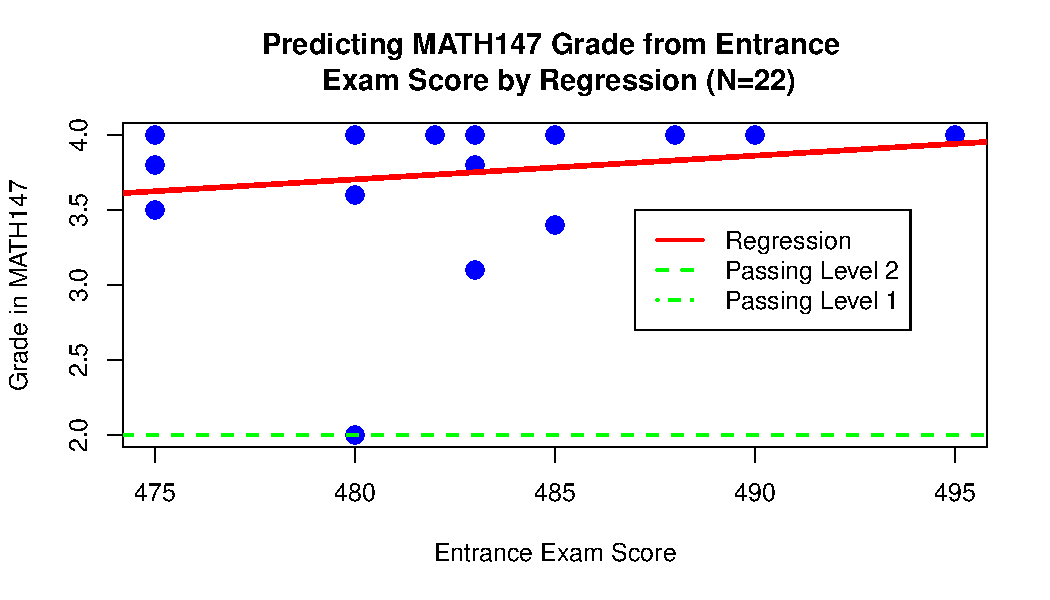
\includegraphics[width=\maxwidth]{figure/147regressiongraph-1} 

\end{knitrout}

\begin{knitrout}
\definecolor{shadecolor}{rgb}{0.969, 0.969, 0.969}\color{fgcolor}
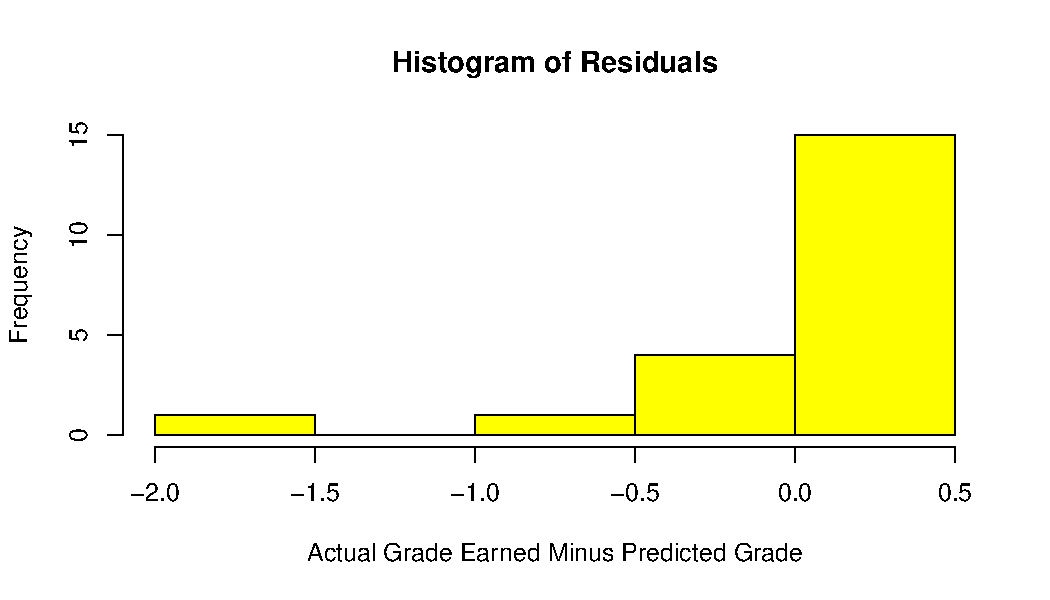
\includegraphics[width=\maxwidth]{figure/147residualsplot-1} 

\end{knitrout}

The regression line predicts a grade of 3.5 for a student earning an Entrance Exam score that is 5 points lower than the current cutoff.


\newpage
\subsection{MATH\&141 - Precalculus 1}


%<<141cutoff, echo=FALSE, fig.height=4>>=
%visualDisplayCutoffData(df1, "MATH&141", 2.0, "MATH097", 2.5, 480, textScale=0.75)
%
%visualDisplayCutoffData(df1, "MATH&141", 1.0, "MATH097", 2.5, 480, textScale = 0.75)
%@


\begin{knitrout}
\definecolor{shadecolor}{rgb}{0.969, 0.969, 0.969}\color{fgcolor}
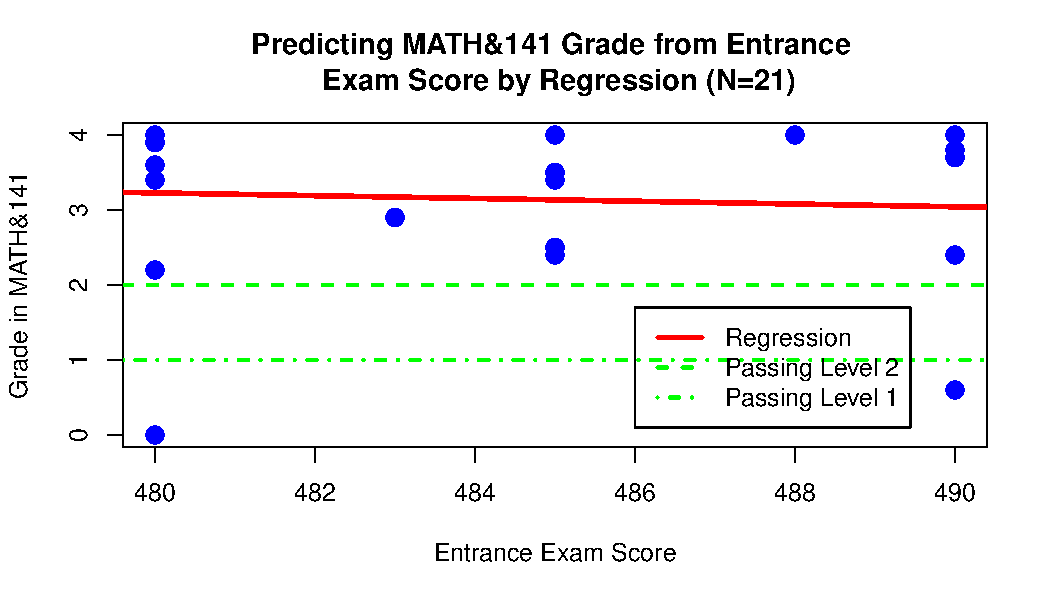
\includegraphics[width=\maxwidth]{figure/141regressiongraph-1} 

\end{knitrout}

\begin{knitrout}
\definecolor{shadecolor}{rgb}{0.969, 0.969, 0.969}\color{fgcolor}
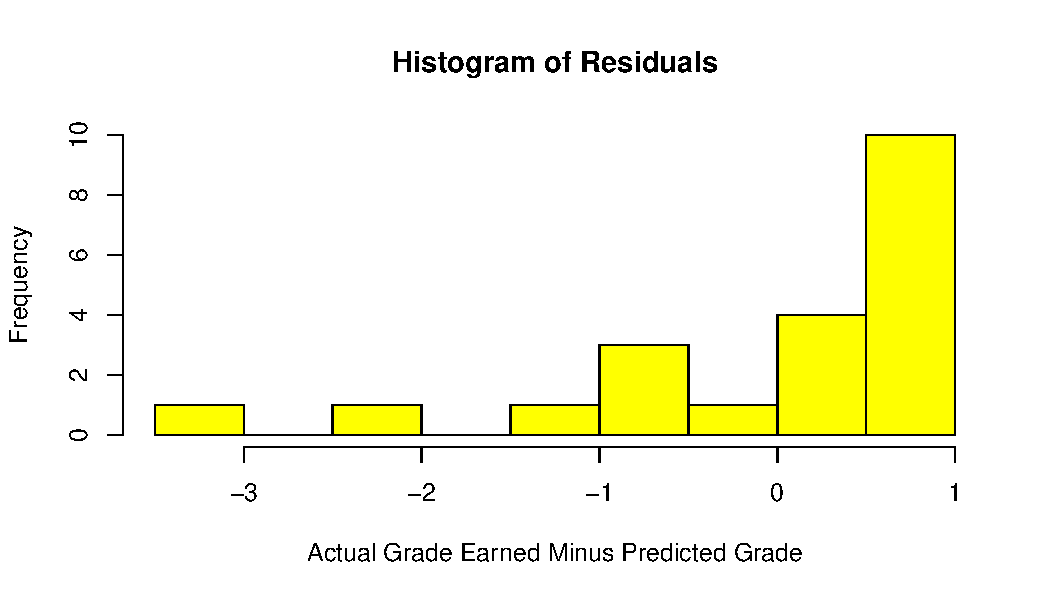
\includegraphics[width=\maxwidth]{figure/141residualsplot-1} 

\end{knitrout}

The regression line predicts a grade of 3.3 for a student earning an Entrance Exam score that is 5 points lower than the current cutoff.


\newpage
\subsection{MATH\&142 - Precalculus 2}


%<<142cutoff, echo=FALSE, fig.height=4>>=
%visualDisplayCutoffData(df1, "MATH&142", 2.9, "MATH&141", 2.0, 575)
%@


\begin{knitrout}
\definecolor{shadecolor}{rgb}{0.969, 0.969, 0.969}\color{fgcolor}
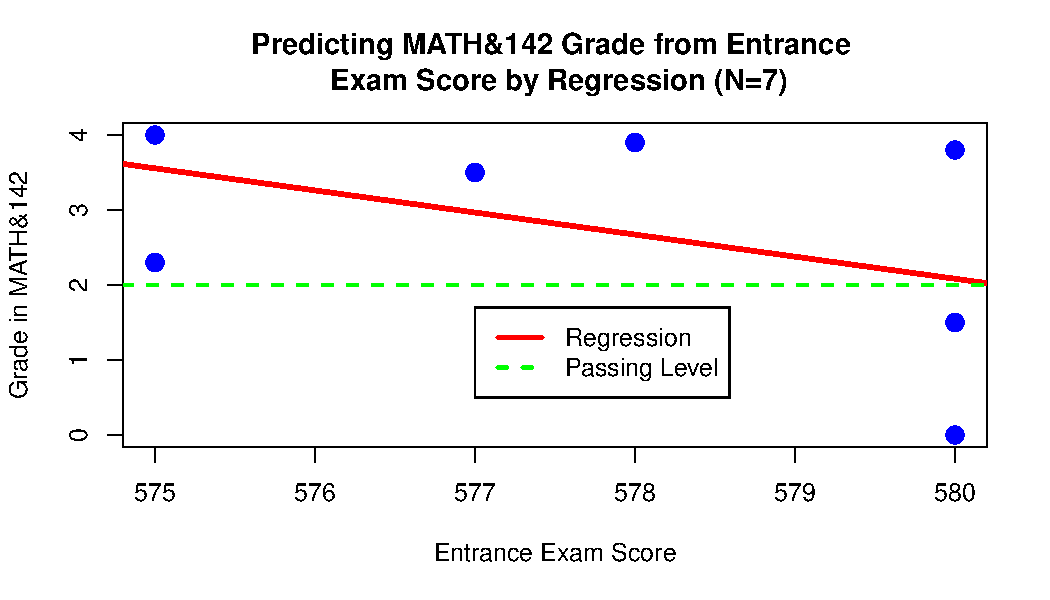
\includegraphics[width=\maxwidth]{figure/142regressiongraph-1} 

\end{knitrout}

\begin{knitrout}
\definecolor{shadecolor}{rgb}{0.969, 0.969, 0.969}\color{fgcolor}
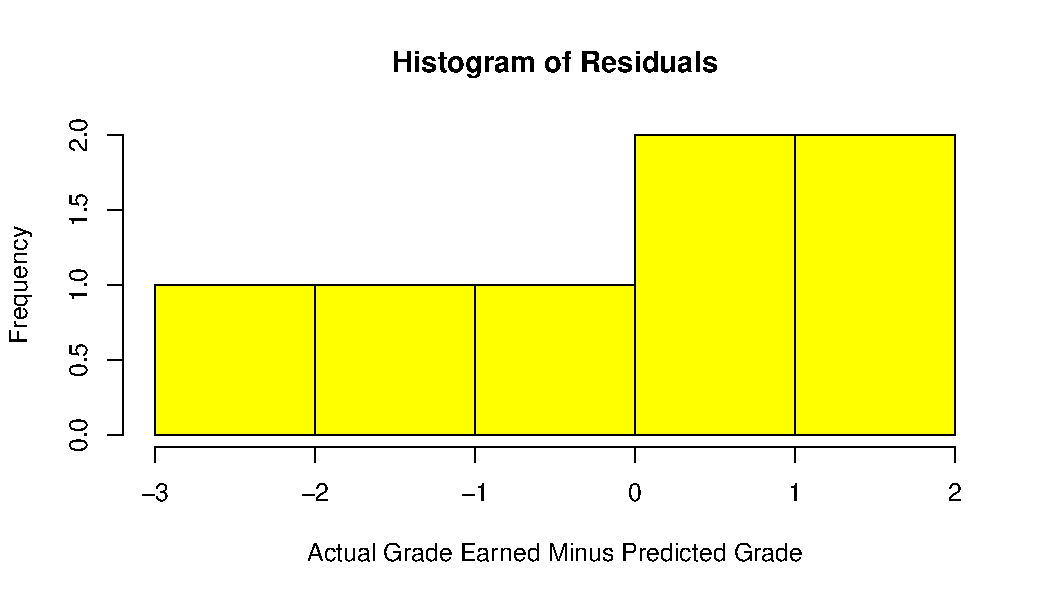
\includegraphics[width=\maxwidth]{figure/142residualsplot-1} 

\end{knitrout}

The regression line predicts a grade of 5 for a student earning an Entrance Exam score that is 5 points lower than the current cutoff.  Of course, the maximum possible grade is 4.0.  The negative slope of this line is likely due to the small sample size and the presence of a single outlier on the bottom right.


\newpage
\subsection{MATH\&151, Calculus 1}


%<<151cutoff, echo=FALSE, fig.height=4>>=
%visualDisplayCutoffData(df1, "MATH&151", 2.0, "MATH&142", 2.0, 675)
%@

\begin{knitrout}
\definecolor{shadecolor}{rgb}{0.969, 0.969, 0.969}\color{fgcolor}
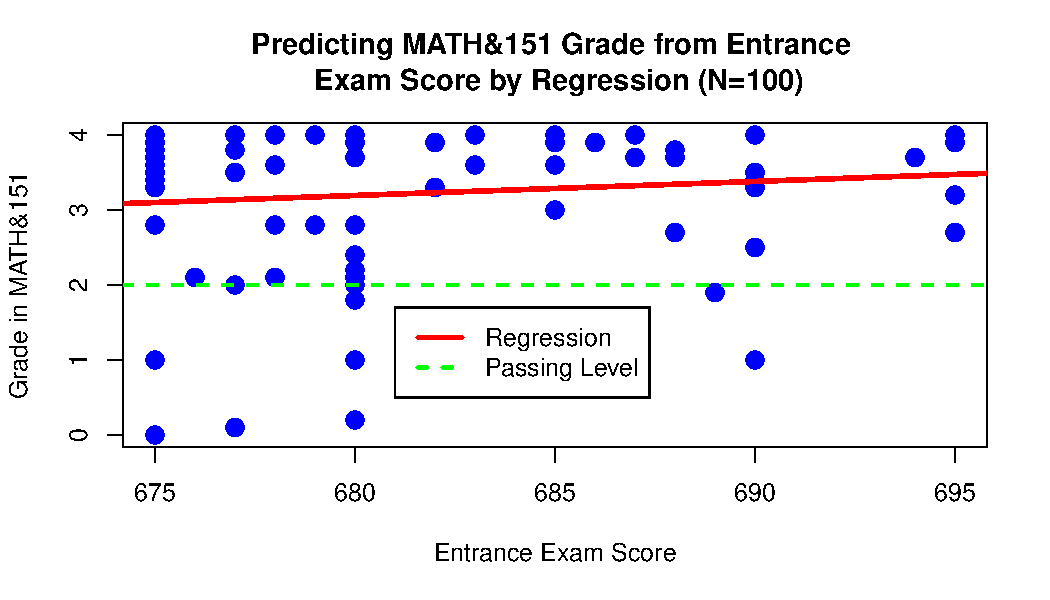
\includegraphics[width=\maxwidth]{figure/151regressiongraph-1} 

\end{knitrout}

\begin{knitrout}
\definecolor{shadecolor}{rgb}{0.969, 0.969, 0.969}\color{fgcolor}
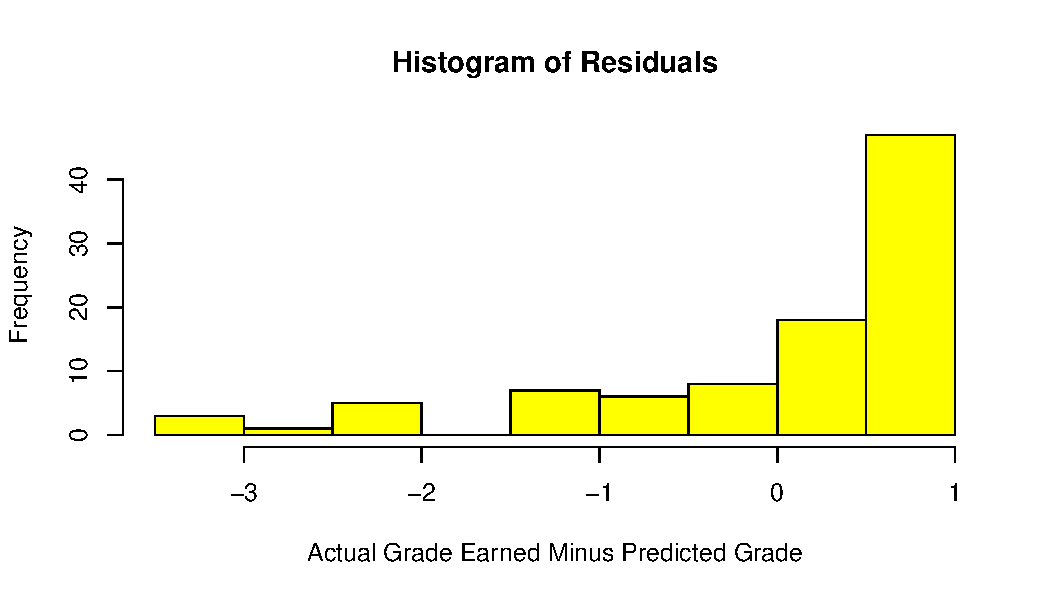
\includegraphics[width=\maxwidth]{figure/151residualsplot-1} 

\end{knitrout}

The regression line predicts a grade of 3 for a student earning an Entrance Exam score that is 5 points lower than the current cutoff.



\newpage
\section{Codebook}

The following information describes the data fields in the ``anonymousdata.csv'' file from which the analysis in this report begins.


\begin{itemize}
\item {\bf X} and {\bf X.1} - These are line numbers for the table and convey no other information.


\item {\bf Course.taken} - Indicates the math course: MATH062 is Arithmetic, MATH070 is Prealgebra, MATH072 is Elementary Algebra, MATH097 is Intermediate Algebra, MATH\&107 is Math in Society, MATH147 is Finite Math for Business and Social Science, MATH\&141 is Precalculus 1, MATH\&142 is Precalculus 2, and MATH\&151 is Calculus 1.

\item {\bf Quarter} - Indicates the quarter in which the course was taken.  The first two digits indicate the acemic year: 01 is 2010-2011, 12 is 2011-2012, 23 is 2012-2013, and 34 is 2013-2014.  The final digit indicates the quarter: 1 is summr, 2 is fall, 3 is winter, and 4 is spring.

\item {\bf Grade.earned} - This is the grade reported on the students' transcript.  Grades are awarded on a scale of 0.0-4.0.  I is Incomplete, N is Audit, NC is No Credit, P is Pass, and W is Withdrawal.


\item {\bf numericalgrade} - This is the same as Grade.earned when the assigned grade is a number in the range 0.0-4.0, and it NA otherwise.

\item {\bf Last.quarter.of.attendance} - Indicates the last quarter during which the student was enrolled; z999 indicates that the student was still enrolled at the time of data collection.

\item {\bf Drop.date} - If the student dropped the course after the 4th day of the quarter, this indicates the date of the withdrawal.

\item {\bf Concurrent.GPA} - Indicates the GPA earned during Quarter, including the grade earned in the math course.

\item {\bf Concurrent.credits.registered.for} - Indicates how many credits a student was registered for during Quarter.

\item {\bf Concurrent.credits.earned} - Indicates how many credits student successfully earned during Quarter.

\item {\bf COMPASS.Reading} - Reading score on COMPASS placement exam.

\item {\bf COMPASS.Number.Skills} - Number Skills score on COMPASS placement exam.

\item {\bf COMPASS.Elem.Alg} - Elementary Algebra score on COMPASS placement exam.

\item {\bf COMPASS.College.Alg.} - College Algebra score on COMPASS placement exam.

\item {\bf COMPASS.Trig} - Trigonometry score on COMPASS placement exam.

\item {\bf MAPS.Score} - Score on Entrance Exam.  The range of the score indicates which exam was attempted: 0-99 indicates that the student tried to test into MATH062 (80 or higher is passing); 100-199 indicates MATH070 (180 or higher is passing), 200-299 indicates MATH072 (280 or higher is passing), 300-399 indicates MATH097 (380 or higher is passing), 400-499 indicates MATH\&107, MATH\&141, or MATH147 (475 or higher is passing for MATH\&107 and MATH147, while 480 or higher is passing for MATH\&141); 500-599 indicates MATH\&142 (575 or higher is passing); 600-699 indicates MATH\&151 (675 or higher is passing).

\item {\bf FID} - Stands for ``Fake ID'', which is a surrogate for the SID (``Student ID'') number which cannot be released to the public because of federal privacy laws.  Two entries in the table will have the same FID number if and only if they correspond to the same student.
\end{itemize}






\section{Code and Data}

The raw data for this analysis included student identification numbers, or SIDs, which cannot be released to the public due to privacy laws.  Therefore, the publicly-available version of this data has had these SIDs stripped and replaced by randomly-generated fake identification numbers (labeled FID in the cleaned data set).  Here is the code that was used for this pre-processing stage:


\begin{knitrout}
\definecolor{shadecolor}{rgb}{0.969, 0.969, 0.969}\color{fgcolor}\begin{kframe}
\begin{alltt}
\hlstd{df1} \hlkwb{=} \hlkwd{read.csv}\hlstd{(}\hlstr{"rawdata/startingData.csv"}\hlstd{)}
\hlstd{df1} \hlkwb{=} \hlkwd{subset}\hlstd{(df1, Grade.earned} \hlopt{!=} \hlstr{"*"}\hlstd{)}
\hlstd{SID} \hlkwb{=} \hlkwd{unique}\hlstd{(df1}\hlopt{$}\hlstd{SID.)}
\hlstd{FID} \hlkwb{=} \hlnum{1}\hlopt{:}\hlkwd{length}\hlstd{(SID)}
\hlkwd{set.seed}\hlstd{(}\hlnum{2014}\hlstd{)}
\hlstd{FID} \hlkwb{=} \hlkwd{sample}\hlstd{(FID)}
\hlstd{SIDtoFID}\hlkwb{=}\hlkwd{cbind}\hlstd{(SID,FID)}
\hlkwd{write.csv}\hlstd{(SIDtoFID,}\hlstr{"cleandata/SIDtranslationtable.csv"}\hlstd{)}
\hlstd{translator} \hlkwb{=} \hlkwd{read.csv}\hlstd{(}\hlstr{"cleandata/SIDtranslationtable.csv"}\hlstd{)}
\hlstd{df1}\hlopt{$}\hlstd{FID} \hlkwb{=} \hlkwd{numeric}\hlstd{(}\hlkwd{length}\hlstd{(df1}\hlopt{$}\hlstd{SID.))}
\hlkwa{for} \hlstd{(k} \hlkwa{in} \hlnum{1}\hlopt{:}\hlkwd{length}\hlstd{(df1}\hlopt{$}\hlstd{SID.))\{}
  \hlstd{tableentry} \hlkwb{=} \hlkwd{match}\hlstd{(df1}\hlopt{$}\hlstd{SID.[k],translator[,}\hlnum{2}\hlstd{])}
  \hlstd{df1}\hlopt{$}\hlstd{FID[k]} \hlkwb{=} \hlstd{translator[tableentry,}\hlnum{3}\hlstd{]}
\hlstd{\}}
\hlstd{df1}\hlopt{$}\hlstd{SID.} \hlkwb{=} \hlkwa{NULL}
\hlstd{df1}\hlopt{$}\hlstd{Last.Name} \hlkwb{=} \hlkwa{NULL}
\hlstd{df1}\hlopt{$}\hlstd{First.Name} \hlkwb{=} \hlkwa{NULL}
\hlstd{df1}\hlopt{$}\hlstd{Date.of.Birth} \hlkwb{=} \hlkwa{NULL}
\hlstd{df1}\hlopt{$}\hlstd{Sex} \hlkwb{=} \hlkwa{NULL}
\hlstd{df1}\hlopt{$}\hlstd{Ethnicity} \hlkwb{=} \hlkwa{NULL}
\hlkwd{write.csv}\hlstd{(df1,} \hlstr{"cleandata/anonymousdata.csv"}\hlstd{)}
\end{alltt}
\end{kframe}
\end{knitrout}

The second line in the code above removes the entries from the data set for which no grade was recorded (there was only one such entry in the entire study).

Two additional preprocessing steps were applied to the data.  First, three columns were added to the data frame to indicate student success at the 1.0, 2.0 and 2.5 grade-point levels.  Second, another column was added in which non-numerical grades were given numerical representations, to facilitate generating some of the graphs found in this report.  The code for that stage of preprocessing is:

\begin{knitrout}
\definecolor{shadecolor}{rgb}{0.969, 0.969, 0.969}\color{fgcolor}\begin{kframe}
\begin{alltt}
\hlstd{df1}\hlopt{$}\hlstd{success1.0} \hlkwb{=} \hlkwd{logical}\hlstd{(}\hlkwd{length}\hlstd{(df1}\hlopt{$}\hlstd{FID))}
\hlstd{df1}\hlopt{$}\hlstd{success1.0[df1}\hlopt{$}\hlstd{numericalgrade} \hlopt{>=} \hlnum{1.0}\hlstd{]} \hlkwb{=} \hlnum{TRUE}
\hlstd{df1}\hlopt{$}\hlstd{success1.0[df1}\hlopt{$}\hlstd{Grade.earned} \hlopt{==} \hlstr{"P"}\hlstd{]} \hlkwb{=} \hlnum{TRUE}

\hlstd{df1}\hlopt{$}\hlstd{success2.0} \hlkwb{=} \hlkwd{logical}\hlstd{(}\hlkwd{length}\hlstd{(df1}\hlopt{$}\hlstd{FID))}
\hlstd{df1}\hlopt{$}\hlstd{success2.0[df1}\hlopt{$}\hlstd{numericalgrade} \hlopt{>=} \hlnum{2.0}\hlstd{]} \hlkwb{=} \hlnum{TRUE}

\hlstd{df1}\hlopt{$}\hlstd{success2.5} \hlkwb{=} \hlkwd{logical}\hlstd{(}\hlkwd{length}\hlstd{(df1}\hlopt{$}\hlstd{FID))}
\hlstd{df1}\hlopt{$}\hlstd{success2.5[df1}\hlopt{$}\hlstd{numericalgrade} \hlopt{>=} \hlnum{2.5}\hlstd{]} \hlkwb{=} \hlnum{TRUE}

\hlstd{df1}\hlopt{$}\hlstd{forcednumericalgrade} \hlkwb{=} \hlstd{df1}\hlopt{$}\hlstd{numericalgrade}
\hlstd{df1}\hlopt{$}\hlstd{forcednumericalgrade[df1}\hlopt{$}\hlstd{Grade.earned} \hlopt{==} \hlstr{"W"}\hlstd{]} \hlkwb{=} \hlopt{-}\hlnum{0.1}
\hlstd{df1}\hlopt{$}\hlstd{forcednumericalgrade[df1}\hlopt{$}\hlstd{Grade.earned} \hlopt{==} \hlstr{"N"}\hlstd{]} \hlkwb{=} \hlopt{-}\hlnum{0.1}
\hlstd{df1}\hlopt{$}\hlstd{forcednumericalgrade[df1}\hlopt{$}\hlstd{Grade.earned} \hlopt{==} \hlstr{"P"}\hlstd{]} \hlkwb{=} \hlnum{1}
\hlstd{df1}\hlopt{$}\hlstd{forcednumericalgrade[df1}\hlopt{$}\hlstd{Grade.earned} \hlopt{==} \hlstr{"NC"}\hlstd{]} \hlkwb{=} \hlopt{-}\hlnum{0.1}
\hlstd{df1}\hlopt{$}\hlstd{forcednumericalgrade[df1}\hlopt{$}\hlstd{Grade.earned} \hlopt{==} \hlstr{"I"}\hlstd{]} \hlkwb{=} \hlopt{-}\hlnum{0.1}


\hlkwd{write.csv}\hlstd{(df1,} \hlstr{"cleandata/preprocessedData.csv"}\hlstd{)}
\end{alltt}
\end{kframe}
\end{knitrout}






All code, including the code used to generate this document, can be found on GitHub at \\https://github.com/kriskissel.  The data files ``anonymousdata.csv'' and ``preprocessedData.csv'' can also be found there.








\end{document}
